\documentclass[14pt, a4paper]{extbook}

%\fontsize{14}{1.25}
\usepackage[T1]{fontenc}
\usepackage[utf8]{inputenc}
\usepackage[russian]{babel}

% margins
%\setlength{\textwidth}{360pt}
%\setlength{\oddsidemargin}{22pt}
%\setlength{\evensidemargin}{70pt}
%\setlength{\marginparwidth}{106pt}

% page margin
%\usepackage[top=2cm, bottom=2cm, left=2cm, right=2cm]{geometry}
\usepackage[left=2cm,right=2cm,top=2cm,bottom=2cm,bindingoffset=0cm]{geometry}

% AMS packages
\usepackage{amsmath}
\usepackage{amssymb}
\usepackage{amsfonts}
\usepackage{amsthm}

% floating option for figures
\usepackage{float}

\usepackage{xcolor}

\usepackage{bbm}

\usepackage{fancyhdr}
\pagestyle{fancy}
% modifying page layout using fancyhdr
\fancyhf{}
\renewcommand{\sectionmark}[1]{\markright{\thesection\ #1}}
\renewcommand{\subsectionmark}[1]{\markright{\thesubsection\ #1}}

\rhead{\fancyplain{}{\rightmark }}
\cfoot{\fancyplain{}{\thepage }}

\usepackage{array}
\usepackage{braket}

\makeatletter
\def\env@dmatrix{\hskip -\arraycolsep
  \let\@ifnextchar\new@ifnextchar
  \extrarowheight=2ex
  \array{*\c@MaxMatrixCols{>{\displaystyle}c}}}

\newenvironment{dmatrix}
  {\env@dmatrix}
  {\endarray\hskip-\arraycolsep}

\newenvironment{bdmatrix}
  {\left[\env@dmatrix}
  {\endmatrix\right]}
\makeatother

\newcommand{\mf}{\mathbf}

\newcommand{\lb}{\left(}
\newcommand{\rb}{\right)}
\newcommand{\lsq}{\left[}
\newcommand{\rsq}{\right]}
\newcommand{\lc}{\left\{}
\newcommand{\rc}{\right\}}

\newcommand{\bbI}{\mathbb{I}}
\newcommand{\bba}{\mathbbm{a}}
\newcommand{\bbA}{\mathbb{A}}
\newcommand{\bbB}{\mathbb{B}}
\newcommand{\bbG}{\mathbb{G}}
\newcommand{\bbM}{\mathbb{M}}
\newcommand{\bbV}{\mathbb{V}}
\newcommand{\bbW}{\mathbb{W}}
\newcommand{\EOmega}{\boldsymbol{\Omega}_{\rm \textbf{e}}}
\newcommand{\mfpe}{\mf{p_e}}
\newcommand{\mfpet}{\mf{p_e^+}}
\newcommand{\mfq}{\mf{q}}
\newcommand{\mfp}{\mf{p}}
\newcommand{\mfJ}{\mf{J}}

\DeclareMathAlphabet{\mymathbb}{U}{BOONDOX-ds}{m}{n}
\newcommand{\bbzero}{\mymathbb{0}}
\newcommand{\bbone}{\mymathbb{1}}

\def\hh{_{\rm H}}

\usepackage[toc]{appendix}

\usepackage{chngcntr}
\usepackage{etoolbox}
\AtBeginEnvironment{subappendices}{%
\chapter*{Appendix}
\addcontentsline{toc}{chapter}{Appendices}
\counterwithin{figure}{section}
\counterwithin{table}{section}
}

\usepackage{mathtools}

\DeclarePairedDelimiter\abs{\lvert}{\rvert}%
\DeclarePairedDelimiter\norm{\lVert}{\rVert}%

% Swap the definition of \abs* and \norm*, so that \abs
% and \norm resizes the size of the brackets, and the 
% starred version does not.
\makeatletter
\let\oldabs\abs
\def\abs{\@ifstar{\oldabs}{\oldabs*}}
%
\let\oldnorm\norm
\def\norm{\@ifstar{\oldnorm}{\oldnorm*}}
\makeatother

\newcommand{\bnp}[1]{b_n^{(#1)}}

% hyperlinks for eqref and cite
\usepackage{hyperref}

% indentation in the first paragraph of section or paragraph
\usepackage{indentfirst}

\newcommand{\boltz}{k_\text{b}}
\newcommand{\kb}{k_\text{b}}
\newcommand{\intty}{\int\limits_{-\infty}^\infty}
\newcommand{\mean}[1]{\langle #1 \rangle}
\newcommand{\bs}{\boldsymbol}
\newcommand{\mL}{\mathcal{L}}
\newcommand{\mH}{\mathcal{H}}
\newcommand{\mN}{\mathcal{N}}
\newcommand{\mHplane}{\mathcal{H}_\text{plane}}
\newcommand{\bbS}{\mathbb{S}}
\newcommand{\bxi}{\boldsymbol{\xi}}
\newcommand{\rfixed}{r_\text{fixed}}

\usepackage[raggedright]{titlesec}
\usepackage{fourier, erewhon}
\usepackage{microtype}
 \SetTracking[no ligatures={f}]{encoding=*}{100}
% changing fontsize of chapter titles
 \titleformat{\chapter}[display]
 {\bfseries\Large\lsstyle\SetTracking[no ligatures = {f}]{encoding = *}{50}\filleft}
 {\MakeUppercase{\chaptername}\enspace\thechapter}
 {2ex}
 {\titlerule[1pt]\vspace{2ex}\MakeUppercase}%
\titlespacing*{\chapter}{0pt}{-60pt}{10ex}

% changing fontsize of section titles
\titleformat{\section}
 {\normalfont\fontsize{16}{15}\bfseries}{\thesection}{1em}{}


\begin{document}

\tableofcontents

\chapter{Введение}
\iffalse
Homonuclear diatomic molecules, which includes several astrophysically and atmo-
spherically relevant species, have zero electric dipole moment due to their inversion
symmetry. This means that these molecules are in principle infrared inactive. How-
ever, gases of apolar molecules exhibit collision-induced absorption, as was first shown
experimentally for a gas of oxygen molecules.[10] This absorption originates from col-
lision complexes present in the gas. The collision complex can be considered to be a
short-lived species, which may have a lower symmetry than the individual molecules
and hence an electric dipole moment. Since these collision complexes are short-lived,
the resulting absorption spectra are typically broad in frequency.

Поглощение света описывается законом Бугера-Ламберта-Бера 
\begin{gather}
    I = I_0 \exp \lb - \alpha l \rb. 
\end{gather}
По закону Бера коэффицициент поглощения $\alpha$ связан линейно с плотностью поглощающего газа $n$
\begin{gather}
    \alpha = \sigma n,
\end{gather}
где через $\sigma$ обозначено сечение поглощения. Зависимость предполагает, что поглощение происходит индивидуальными молекулами. В общем случае, для описания этой зависимости может быть использовано вириальное разложение
\begin{gather}
    \alpha = \sigma n + \alpha_\text{binary} n^2 + \alpha_\text{ternary} n^3 + O(n^4), 
\end{gather}
в котором квадратичное слагаемое описывает столкновительно-индуцированное поглощение бинарными комплексами, кубическое слагаемое -- тройными комплексами, и т.д. Стоит отметить, что сечение поглощения мономера $\sigma$ зависит от давления (проявляется это, например, в сдвигах и уширениях линий), поэтому при каждой фиксированной частоте поглощение мономера не является линейным по плотности $n$, однако интегральная интенсивность линейна по плотности. \par
Таким образом, для моделирования суммарного профиля поглощения необходимо знать сечение поглощения $\sigma$, коэффициент бинарного поглощения $\alpha_\text{binary}$, и т.д., и как эти эти величины зависят от атмосферных характеристик, таких как температура. Данная работа посвящена расчет коэффициентов бинарного поглощения $\alpha_\text{binary}$ для различных систем, имеющих практическую значимость в атмосферных приложениях. \par
Спектры плотных газов и газовых смесей существенно отличаются от спектров, зарегистрированных при низких плотностях. По мере увеличения плотности, наблюдается линейное увеличение интенсивностей разрешенных колебательно-вращательных и электронных полос. При промежуточных значениях плотности могут возникнуть новые полосы поглощения, которые не наблюдались при более низких плотностях, причем интенсивность этих полос (по крайней мере в первом приближении) может быть описана квадратичным или кубическим законом. За появление этих полос отвественны ван дер Ваальсовы комплексы двух или большего количества молекул. Подобные полосы поглощения найдены во многих молекулярных газах, даже молекулы которых не обладают постоянным дипольным моментом.  

Состояния ван дер Ваальсовых комплексов классифицируют на связанные, полная колебательно-вращательная энергия меньше энергии диссоциации, и свободные. 

Впервые квадратичную зависимость коэффициента поглощения от плотности наблюдал Йенсен (Janssen) в 1885 году на полосах поглощениях кислорода \cite{janssen1885}.
\fi


\chapter{Теоретическое введение}
\section{Взаимодействие электромагнитного излучения с молекулярными системами}
Рассмотрим систему из $N$ взаимодействующих частиц (молекул) в квантовом состоянии $\ket{j}$. Обозначим гамильтониан системы через $\hat{H}_0$. Пусть система подвергается воздействию электрического поля частоты $\omega$, которое индуцирует переходы в другие состояния системы $\ket{k}$ при условии, что частота поля близка к частотам Бора системы
%
\begin{gather}
    \omega_{jk} = (E_j - E_k) / \hbar.
\end{gather}

Будем считать, что длина волны рассматриваемого поля $\lambda$ много больше размеров молекул в системе, поэтому в локальной окрестности молекул поле можно считать однородным в пространстве.  Электрическая составляющая электромагнитной волны может быть записана в виде суммы
%
\begin{gather}
    \mf{E}(t) = E_0 \boldsymbol{\varepsilon} \cos \omega t = \frac{E_0 \boldsymbol{\varepsilon}}{2} \lb e^{i \omega t} + e^{- \omega t} \rb,
\end{gather}
%
где $E_0$ -- амплитуда волны, а $\boldsymbol{\varepsilon}$ -- единичный вектор, направленный вдоль направления распространения волны. Энергия взаимодействия молекулярной системы с электрическим полем в дипольном приближении равна
%
\begin{gather}
    W(t) = - (\boldsymbol{\mu} \cdot \mf{E}) = - \frac{E_0}{2} \lb \boldsymbol{\mu} \cdot \boldsymbol{\varepsilon} \rb \lsq e^{i \omega t} + e^{-i \omega t} \rsq, \label{part1-dipole-approximation} 
\end{gather}
%
где через $\boldsymbol{\mu}$ обозначен полный дипольный момент системы. Взаимодействие молекулярных систем с электромагнитным полем часто рассматривают в этом приближении, считая поле классическим объектом. Уравнение \eqref{part1-dipole-approximation} подразумевает, что взаимодействие между полем и молекулярной системой исчезает, когда напряженность поля $\mf{E}$ равна 0. Однако это не так, иначе бы не наблюдалось явления спонтанного излучения. Связь между электромагнитным полем и системой должна быть двухсторонней, наличие поля может вызывать изменения в состоянии системы, но и наличие системы может изменять состояние поля. \par  
Взаимодействие молекулярных систем с электрическим полем традиционно рассматривается в рамках временной теории возмущений \cite{cohentanuji, greiner}. Согласно приложению А, вероятность индуцированного возмущением $W(t)$ перехода между состояниями невозмущенной системы $\ket{j} \rightarrow \ket{k}$ в первом порядке временной теории возмущения равна
%
\begin{gather}
    \mathcal{P}_{jk}(t) = \frac{1}{\hbar^2} \abs{ \int\limits_0^t W_{jk}(t^\prime) e^{i \omega_{jk} t^\prime} dt^\prime }^2,
\end{gather}
%
где через $W_{jk}(t)$ обозначен матричный элемент возмущения на состояниях невозмущенной системы, равный в данном случае
%
\begin{gather}
    W_{jk} = -\frac{E_0}{2} \bra{j} \boldsymbol{\mu} \cdot \boldsymbol{\varepsilon} \ket{k} \lsq e^{i \omega t} + e^{-i \omega t} \rsq.
\end{gather}

Коэффициенты разложения первого порядка $b_n^{(1)}(t)$ возмущенной волновой функции $\ket{\psi(t)}$ в базисе собственных функций невозмущенного гамильтониана равны (см. соотношение \eqref{app-expansion})
\begin{gather}
    b_{n}^{(1)}(t; \omega) = -\frac{E_0}{2 \hbar} \bra{j} \boldsymbol{\mu} \cdot \boldsymbol{\varepsilon} \ket{k} \lsq \frac{e^{i (\omega_{jk} + \omega) t} - 1}{\omega_{jk} + \omega} + \frac{e^{i (\omega_{jk} - \omega) t} - 1}{\omega_{jk} - \omega} \rsq. \label{part1-bn-expression}
\end{gather}
%
Квадрат модуля коэффициента $b_{n}^{(1)}$ определяет вероятность перехода в $n$-ое стационарное состояние невозмущенного гамильтониана. Возводя в квадрат выражение \eqref{part1-bn-expression}, после алгебраических преобразований приходим к
%
\begin{gather}
    \hspace*{-0.5cm}
    \abs{b_{n}^{(1)}(t)}^2 = \frac{E_0}{\hbar^2} \lsq \frac{\sin^2 \lb \frac{1}{2} \lb \omega_{jk} + \omega \rb t \rb}{\lb \omega_{jk} + \omega \rb^2} + \frac{\sin^2 \lb \frac{1}{2} \lb \omega_{jk} - \omega \rb t \rb}{\lb \omega_{jk} - \omega \rb^2} + \frac{ 8 \cos \lb \omega t \rb \sin \lb \frac{1}{2} \lb \omega_{jk} + \omega \rb t \rb \sin \lb \frac{1}{2} \lb \omega_{jk} - \omega \rb t \rb}{\lb \omega_{jk} + \omega \rb \lb \omega_{jk} - \omega \rb} \rsq. \label{part1-bn-expression2}
\end{gather}
 
В данном контексте нас интересуют не вероятности переходов, а скорости переходов $\Gamma_{jk}$ (иными словами, вероятности $P_{jk}$, отнесенные к единице времени) при больших значениях $t$
%
\begin{gather}
    \Gamma_{jk} = \lim_{t \rightarrow \infty} \frac{P_{jk}}{t}.
\end{gather}
%
При предельном переходе в \eqref{part1-bn-expression2} первые два слагаемые преобразуются к дельта-функционалам, в то время как последнее слагаемое оказывается нулевым \cite{baym-quantum-mechanics}. Итак, выражение для скорости переходов оказывается следующим \cite{mcquarrie-statistical-mechanics}  
%
\begin{gather}
    \Gamma_{jk} = \frac{\pi E_0^2}{2 \hbar^2} \abs{ \bra{j} \boldsymbol{\mu} \cdot \boldsymbol{\varepsilon} \ket{k} }^2 \Big[ \delta \lb \omega_{jk} - \omega \rb + \delta \lb \omega_{jk} + \omega \rb \Big]. \label{part1-transition-rate} 
\end{gather}

Выражение \eqref{part1-transition-rate} определяет скорость переходов между конкретными состояниями невозмущенной системы $\ket{j}$ и $\ket{k}$. Скорость поглощения энергии в ходе переходов между этими состояниями равна $\hbar \omega_{jk} \Gamma_{jk}$, т.к. в ходе одно акта поглощения, система поглощает энергию, равную $\hbar \omega_{jk}$. Скорость поглощения энергии в ходе переходов с заданного уровня $\ket{j}$ может быть получена при суммировании по всем состояниям $\ket{k}$, которые доступны системе для перехода. Наконец, суммарная скорость поглощения излучения системой $-\dot{E}_\text{rad}$ получается в результате суммирования по всем возможным начальным состояниям $\ket{j}$ с соответствующими заселенностями $\rho_j$
\begin{gather}
    -\dot{E}_\text{rad} = \sum_j \sum_k \rho_j \hbar \omega_{jk} \Gamma_{jk} = \frac{\pi E_0^2}{2 \hbar} \sum_{j, k} \omega_{jk} \rho_j \abs{ \bra{j} \boldsymbol{\mu} \cdot \boldsymbol{\varepsilon} \ket{k} }^2 \Big[ \delta \lb \omega_{jk} - \omega \rb + \delta \lb \omega_{jk} + \omega \rb \Big]. \label{part1-energy-absorption-rate}
\end{gather}

Для получения более симметричной формы уравнения \eqref{part1-energy-absorption-rate} осуществим алгебраические преобразования. Рассмотрим отдельно вторую сумму, получающуюся при раскрытии скобок в уравнении \eqref{part1-energy-absorption-rate}. Поменяем местами индексы $j \leftrightarrow k$, что обосновывается тем, что оба индекса пробегают по всем квантовым состояниям системы,
\begin{gather}
    \frac{\pi E_0^2}{2 \hbar} \sum_{j, k} \omega_{jk} \rho_j \abs{ \bra{j} \boldsymbol{\mu} \cdot \boldsymbol{\varepsilon} \ket{k} }^2 \delta \lb \omega_{jk} + \omega \rb = -\frac{\pi E_0^2}{2 \hbar} \sum_{j, k} \omega_{jk} \rho_j \abs{ \bra{j} \boldsymbol{\mu} \cdot \boldsymbol{\varepsilon} \ket{k} }^2 \delta \lb \omega_{jk} - \omega \rb. \label{part1-index-change}
\end{gather}

Подстановка \eqref{part1-index-change} в \eqref{part1-energy-absorption-rate} приводит к выражению, в котором индексы $j$ и $k$ входят симметричным образом 
%
\begin{gather}
    -\dot{E}_\text{rad} = \frac{\pi E_0^2}{2 \hbar} \sum_{j, k} \omega_{j k} \lb \rho_j - \rho_k \rb \abs{ \bra{j} \boldsymbol{\mu} \cdot \boldsymbol{\varepsilon} \ket{k} }^2 \delta \lb \omega_{jk} - \omega \rb.
\end{gather}

Предположим, что возмущение достаточно слабо и действует на протяжении малого промежутка времени, таким образом, что в любой момент система находится в состоянии теплового равновесия при температуре $T$. Используя это предположение, выразим заселенность $k$-ого состояния через заселенность $j$-го состояния (понятно, что можно воспользоваться и обратной связью, т.к. мы специально привели формулу к симметричному виду относительно замены индексов)
%
\begin{gather}
    \rho_k = \rho_j \exp \lb - \beta \hbar \omega_{jk} \rb,
\end{gather}
%
где $\beta = \boltz T$ и $\boltz$ -- постоянная Больцмана. Кроме того, вследствие того, что внутри суммы находятся дельта-функционалы, центрированные на $\omega_{jk}$ , функции от $\omega$, вычисленные при частоте $\omega_{jk}$, могут быть вынесены из под знака суммы: 
\begin{align}
    -\dot{E}_\text{rad} &= \frac{\pi E_0^2}{2 \hbar} \sum_{j, k} \omega_{jk} \rho_j \lb 1 - \exp \lb - \beta \hbar \omega_{jk} \rb \rb \abs{ \bra{j} \boldsymbol{\mu} \cdot \boldsymbol{\varepsilon} \ket{k} }^2 \delta \lb \omega_{jk} - \omega \rb = \\
    &= \frac{\pi E_0^2}{2 \hbar} \omega \lb 1 - \exp \lb - \beta \hbar \omega \rb \rb \sum_{j, k} \rho_j \abs{ \bra{j} \boldsymbol{\mu} \cdot \boldsymbol{\varepsilon} \ket{k} }^2 \delta \lb \omega_{jk} - \omega \rb. 
\end{align}

Суммарный поток энергии $I$, переносимой электромагнитной волной через среду с показателем преломления $n$, равен усредненному по времени модулю вектора Пойнтинга $\langle S \rangle$ и равен \cite{landau-volume2}
\begin{gather}
    I = \langle S \rangle = \frac{c}{8 \pi} n E_0^2,
\end{gather}
%
где $c$ -- скорость света в вакууме. Показатель поглощения среды $\alpha(\omega)$ определяют как отношение энергии, поглощаемой средой в единицу времени при частоте $\omega$, к энергии, переносимой электромагнитной волной в единицу времени \cite{mcquarrie-statistical-mechanics}
\begin{gather}
    \alpha(\omega) = \frac{-\dot{E}_\text{rad}}{I} = \frac{4 \pi^2}{\hbar c n} \omega \lb 1 - e^{- \beta \hbar \omega} \rb \sum_{j, k} \rho_j \abs{ \bra{j} \boldsymbol{\mu} \cdot \boldsymbol{\varepsilon} \ket{k}}^2 \delta \lb \omega_{jk} - \omega \rb. \label{part1-absorption-coefficient-definition}
\end{gather}

На основании выражения \eqref{part1-absorption-coefficient-definition} определяют \textit{спектральную функцию} $J(\omega)$ \cite{gordon1968}
\begin{gather}
    J(\omega) = \frac{3 \hbar c n \alpha(\omega)}{4 \pi^2 V \omega \lb 1 - e^{-\beta \hbar \omega} \rb} = 3 \sum_{j, k} \rho_j \abs{ \bra{j} \boldsymbol{\mu} \cdot \boldsymbol{\varepsilon} \ket{k} }^2 \delta \lb \omega_{jk} - \omega \rb. \label{part1-spectral-function-definition}
\end{gather}

Отметим, что обычно спектральную функцию определяют таким образом, чтобы ее интеграл по частотному диапазону был равен единице. Здесь принято несколько иное определение, эта функция не нормирована. \par
Альтернативную форму выражения \eqref{part1-spectral-function-definition} получают осуществляя смену Шредингеровского представления квантовой механики на представление Гейзенберга. Состояния в представлении Гейзенберга не зависят от времени -- временная эволюция заложена в операторах. Эволюция оператора $\hat{A}(t)$ описывается оперетором эволюции $U(t)$
\begin{gather}
    \hat{A}(t) = U^{+}(t) A(0) U(t) = e^{\frac{i}{\hbar} H t} \hat{A}(0) e^{-\frac{i}{\hbar} H t}. 
\end{gather}

Удобно перейти в выражении \eqref{part1-spectral-function-definition} к представлению Гейзенберга, представив дельта-функционал как Фурье-образ мнимой экспоненты
\begin{gather}
    \delta (\omega) = \frac{1}{2\pi} \int\limits_{-\infty}^\infty e^{i \omega t} dt,
\end{gather}
получаем
\begin{gather}
    J(\omega) = \frac{3}{2\pi} \sum_{j,k} \rho_j \bra{j} \boldsymbol{\mu} \cdot \varepsilon \ket{k} \bra{k} \boldsymbol{\mu} \cdot \boldsymbol{\varepsilon} \ket{j} \int\limits_{-\infty}^\infty \exp \lsq \lb \frac{E_j - E_k}{\hbar} - \omega \rb t \rsq dt. \label{part1-spectral-function-2}
\end{gather}

Т.к. состояния $\ket{k}$ и $\ket{j}$ являются собственными состояниями гамильтониана $\hat{H}_0$, то
\begin{gather}
    \exp \lb -\frac{i}{\hbar} E_j t \rb \ket{j} = \exp \lb -\frac{i}{\hbar} \hat{H}_0 t \rb \ket{j}, \quad \exp \lb \frac{i}{\hbar} E_k t \rb \bra{k} = \exp \lb \frac{i}{\hbar} \hat{H}_0 t \rb \bra{k}. 
\end{gather}

Произведение матричного элемента и экспоненты с Боровской частотой, получаемое при внесении матричного элемента под интеграл в \eqref{part1-spectral-function-2}, легко переводится в представление Гейзенберга
\begin{gather}
    \exp \lb \frac{i}{\hbar} \lb E_k - E_j \rb t \rb \bra{k} \boldsymbol{\mu} \cdot \boldsymbol{\varepsilon} \ket{j} = \bra{k} \exp \lb \frac{i}{\hbar} \hat{H}_0 t \rb \boldsymbol{\mu} \cdot \boldsymbol{\varepsilon} \exp \lb -\frac{i}{\hbar} \hat{H}_0 t \rb \ket{j} = \bra{k} \boldsymbol{\mu}(t) \cdot \boldsymbol{\varepsilon} \ket{j}. \label{part1-matrix-element}
\end{gather}

Подставляя \eqref{part1-matrix-element} в \eqref{part1-spectral-function-2}, приходим к
\begin{gather}
    J(\omega) = \frac{3}{2\pi} \int\limits_{-\infty}^\infty \sum_{j,k} \rho_j \bra{j} \boldsymbol{\mu} \cdot \boldsymbol{\varepsilon} \ket{k} \bra{k} \boldsymbol{\mu}(t) \cdot \boldsymbol{\varepsilon} \ket{j} e^{-i \omega t} dt.
\end{gather}

Заметим, что суммирование по состояниям $\ket{k}$ может быть устранено, так как его можно выделить как соотношение замкнутости \eqref{app-completeness}. 
\begin{gather}
    J(\omega) = \frac{3}{2\pi} \int\limits_{-\infty}^\infty \sum_j  \rho_{j} \bra{j} \boldsymbol{\mu}(0) \cdot \boldsymbol{\varepsilon} \cdot \boldsymbol{\mu}(t) \cdot \boldsymbol{\varepsilon} \ket{j} e^{-i\omega t} dt.
\end{gather}

Сумма в подынтегральном выражении является квантово-механическим средним по ансамблю значением оператора, которое в дальнейшем будем обозначать через $\langle \cdots \rangle$. Считая среду изотропной, проинтегрируем по всем возможным ориентациям $\boldsymbol{\varepsilon}$:
\begin{gather}
    J(\omega) = \frac{1}{2\pi} \intty \mean{ \bs{\mu}(0) \cdot \bs{\mu}(t) } e^{-i \omega t} dt. \label{litreview-spectral-function}
\end{gather}

Итак, спектральная функция является Фурье-образом автокорреляционной функции оператора дипольного момента поглощающих молекул \cite{gordon1968}. \par
Следует подчеркнуть, что никаких приближений, касающихся характера движения диполей в этом рассмотрении сделано не было. Движение системы полностью обусловлено уравнениями движения, определяемыми гамильтонианом системы $\hat{H}_0$. 

\section{Теория временных функций корреляции и спектральных моментов} \label{section:correlation_functions}

Теория корреляционных функций получила широкое развитие для описания неравновесных систем \cite{zwanzig1965}, однако ее применение к равновесным систем также является очень продуктивным. В системах, находящихся в термодинамическом равновесии, макроскопические параметры не претерпевают эволюции во времени, таким образом для них не имеет смысла вводить какой-то точки отсчета времени. Однако, часто рассматривают условные вероятности, такие как $P(B, t_2 \vert A, t_1) dB$ -- вероятность того, что динамическая переменная $B$ примет значение в диапазоне $(B, \dots, B + dB)$ в момент времени $t_2$ при условии, что другая динамическая переменная имела значение $A$ в момент времени $t_1$ \cite{nitzan2006}. Также можно рассмотреть совместную вероятность $P(B, t_2; A, t_1) dB dA$ -- вероятность того, что переменная $A$ примет значение в диапазоне $(A, \dots, A+dA)$ в момент времени $t_1$ и переменная $B$ примет значение в диапазоне $(B, \dots B+dB)$ в момент времени $t_2$. Эти две вероятности связаны соотношением (формулой полной вероятности)
\begin{gather}
    P(B, t_2; A, t_1) = P(B, t_2 \vert A, t_1) P(A, t_1), 
\end{gather}
где $P(A, t_1) dA$ --вероятность того, что переменная $A$ примет значение в диапазоне $(A, \dots, A+dA)$ в момент времени $t_1$. В стационарных системах последняя вероятность, очевидно, не зависит от времени $P(A, t_1) = P(A)$; условная и совместная вероятности зависят только от разности времени
\begin{gather}
    P(B, t_2; A, t_1) = P(B, t_2 - t_1; A, 0); \quad P(B, t_2 \vert A, t_1) = P(B, t_2 - t_1 \vert A, 0),
\end{gather}
%
где $t = 0$ было положено произвольным образом.\par
Временную корреляционную функцию двух динамических переменных $A$ и $B$ определяют, как интеграл следующего вида 
\begin{gather}
    C_{AB}(t_1, t_2) = \mean{ A(t_1) B(t_2) } = \iint dA dB AB P(B, t_2; A, t_1). \label{part1-correlation-function-definition}
\end{gather}

В стационарных системах функция корреляции суть функция разности времен
\begin{gather}
    \mean{ A(t_1) B(t_2) } = \mean{ A(0) B(t) } = \mean{ A(-t) B(0) }, \quad t = t_2 - t_1.
\end{gather}

С точки зрения классической механики динамические переменные $A$, $B$ являются функциями координат $\mf{r}(t)$ и импульсов $\mf{p}(t)$ всех частиц системы
\begin{gather}
    A(t) = A \lb \mf{r}(t), \mf{p}(t) \rb, \quad B(t) = B \lb \mf{r}(t), \mf{p}(t) \rb.
\end{gather}

Фазовая траектория $\mf{r}(t)$, $\mf{p}(t)$ однозначно определена начальными условиями $\mf{r}(0)$, $\mf{p}(0)$. Таким образом, совместная вероятность в \eqref{part1-correlation-function-definition} определяется функцией распределения $f(\mf{r}, \mf{p})$ начальных условий для фазовых траекторий
\begin{gather}
    C_{AB}(t_1, t_2) = \int d\mf{r} \, d\mf{p} \, f \lb \mf{r}, \mf{p} \rb A\lb t_1; \mf{r}, \mf{p}, t = 0 \rb B \lb t_2; \mf{r}, \mf{p}, t = 0 \rb;
\end{gather}
%
обозначение $A(t_1; \mf{r}, \mf{p}, t = 0)$ означает, что динамическая переменная $A$ в момент времени $t_1$ вычисляется как функция координат и импульсов $A(\mf{r}(t_1), \mf{p}(t_1)$, вычисленных в момент времени $t_1$. \par
    При $t \rightarrow 0$ корреляционная функция $C_{AB}(t)$ становится средним значением произведения динамических переменных $A$ и $B$
\begin{gather}
    C_{AB}(0) = \mean{AB}.
\end{gather}
%
В другом пределе $t \rightarrow \infty$ можно предположить, что корреляция между переменными исчезает, то есть
\begin{gather}
    \lim_{t \rightarrow \infty} C_{AB}(t) = \mean{A} \mean{B}.
\end{gather}

Часто, обьем системы, появляющийся в формуле \eqref{part1-absorption-coefficient-definition}, рассматривают как часть спектральной функции $J(\omega)$ или рассматривают их произведение совместно. Поэтому в соответствии с обозначениями, используемыми в \cite{frommhold}, определим автокорреляционную функцию дипольного момента $C(t)$ как
\begin{gather}
    C(t) = \frac{V}{2\pi} \mean{\bs{\mu}(0) \cdot \bs{\mu}(t)}.
\end{gather}

Спектральная функция \eqref{litreview-spectral-function} принимает действительные значения, следовательно
\begin{gather}
    J(\omega) = J^+(\omega) = \intty C(t)^+ e^{i \omega t} dt = \intty C(-t)^+ e^{-i\omega t} dt, \label{litreview-time-inversion}
\end{gather}
%
где была сделана замена переменной $t \rightarrow -t$, а индекс $+$ обозначает комплексное сопряжение. Сранивая \eqref{litreview-time-inversion} с \eqref{litreview-spectral-function}, получаем
\begin{gather}
    C(t) = C(-t)^+.
\end{gather}

Если мы разложим корреляционную функцию на действительную и мнимую часть, то получим следующие соотношения 
\begin{gather}
    \text{Re} \, C(t) = \text{Re} \, C(-t), \quad \text{Im} \, C(t) = -\text{Im} \, C(t).
\end{gather}

То есть, действительная часть корреляционной функции является четной функции времени, а мнимая часть -- нечетной. Так как классические корреляционные функции являются действительными функциями, то они должны быть четными функциями времени. Квантово-механические же корреляционные функции, как правило, являются комплексными функциями, мнимая часть является исключительно квантово-механическим вкладом, отсутствующим при классическом рассмотрении.


Как уже отмечалось, корреляционные функции в равновесных системах зависят только от разности времени $t_1 - t_2$. Следовательно,
\begin{gather}
    0 = \frac{d}{ds} \mean{ A(t+s) B(s) } = \mean{ \dot{A}(t+s) B(s) } + \mean{ A(t+s) \dot{B}(s) } = \mean{ \dot{A}(t) B(0) } + \mean{ A(t) \dot{B}(0) }.
\end{gather}

Получаем следующее соотношение 
\begin{gather}
    \mean{\dot{A}(t)B(0)} = -\mean{A(t)\dot{B}(0)}, 
\end{gather}
которое для автокорреляционных функций переходит в 
\begin{gather}
    \mean{A \dot{A}} = 0. \label{litreview-temp1}
\end{gather}

Разложим автокорреляционную функцию в ряд по степеням времени $t$
\begin{gather}
    \mean{A(0) A(t)} = \Bigg\langle A(0) \lsq A(0) + t \dot{A}(0) + \frac{t^2}{2!} \ddot{A}(0) + \dots \rsq \Bigg\rangle = \mean{A(0) A(0)} + t \mean{A(0) \dot{A}(0)} + \frac{t^2}{2!} \mean{A(0) \ddot{A}(0)} + \dots \label{litreview-correlation-function-series}
\end{gather}

Отметим, что коэффициенты перед степенями $t^n$ не требуют знания динамики $A(t)$, а являются средними по ансамблю, т.к. временные производные могут быть записаны через скобку Пуассона
\begin{gather}
    \frac{dA}{dt} = \lsq A, H \rsq = \sum_k \lsq \frac{\partial A}{\partial x_k} \frac{\partial H}{\partial p_k} - \frac{\partial A}{\partial p_k} \frac{\partial H}{\partial x_k} \rsq. \label{litreview-poisson-bracket}.
\end{gather}

Соотношение \eqref{litreview-temp1} соотносится с тем, что корреляционная функция является четной функцией. Из четности функции следует, что все коэффициенты перед нечетными степенями $t$ в \eqref{litreview-correlation-function-series} обращаются в ноль. В квантово-механической корреляционной функции нечетные степени не исчезают и, более того, именно за счет них корреляционная функция обладает мнимой частью. \par
Коэффициенты в ряду по степеням времени \eqref{litreview-correlation-function-series} имеют физический смысл моментов соответствующего частотного спектра. Разрешим соотношение \eqref{litreview-spectral-function} относительно автокорреляционной функции дипольного момента и разложим комплексную экспоненту в подынтегральной функции в ряд
\begin{gather}
    C(t) = \frac{1}{2\pi} \intty J(\omega) e^{i \omega t} d \omega = \sum_{n = 0}^\infty \frac{\lb i t\rb^n}{n!} \intty \omega^n J(\omega) d\omega. 
\end{gather}
%
Величины
\begin{gather}
    M_n = \intty \omega^n J(\omega) d\omega \label{litreview-spectral-function-moments}
\end{gather}
%
называют $n$-ыми спектральными моментами. Теоретически, знание всех спектральных моментов эквивалентно знанию спектральной функции (так называемая проблема моментов), однако на практике моменты выше второго находят редко. \par
Итак, спектральные моменты являются моментами спектральной функции и производными автокорреляционной функции дипольного момента в точке $t = 0$
\begin{gather}
    \frac{d^n C}{dt^n} \Bigg\vert_{t = 0} = i^n M_n,
\end{gather}
%
что позволяет вычислить их как средние значения по фазовому пространству. Подробно рассматривать вопрос вычисления спектральных моментов рассматривать не будем, приведем лишь выражения, по которым они могут быть рассчитаны:
\begin{gather}
    M_0 = \frac{\displaystyle \int \bs{\mu}^2 \exp \lsq -H(\mf{q}, \mf{p}) / \kb T \rsq d\mf{q} \, d\mf{p}}{\displaystyle \int \exp \lsq -H(\mf{q}, \mf{p}) / \kb T \rsq d\mf{q} \, d\mf{p}}, \\ 
    M_2 = \frac{\displaystyle \int \dot{\bs{\mu}}^2 \exp \lsq -H(\mf{q}, \mf{p}) / \kb T \rsq d\mf{q} \, d\mf{p}}{\displaystyle \int \exp \lsq -H(\mf{q}, \mf{p}) / \kb T \rsq d\mf{q} \, d\mf{p}},
\end{gather}
%
где производную по времени дипольного момента $\dot{\bs{\mu}}$ в выражении для второго спектрального момента следует преобразовать в скобку Пуассона \eqref{litreview-poisson-bracket}. \par
В данной работе мы вычисляем спектральные моменты по фазовому пространству для контроля сходимости траекторного расчета. В траекторном расчете мы получаем спектральную функцию $J(\omega)$, моменты которой \eqref{litreview-spectral-function-moments}, должны совпасть с моментами по фазовому пространству (конечно, если бы использованы одинаковые поверхности потенциальной энергии и индуцированного дипольного момента). 
\begin{subappendices}
\section{Временная теория возмущений.}

Представленное ниже изложение основано на \cite{cohentanuji}. Рассмотрим физическую систему, описываемую гамильтонианом $\hat{H}_0$; пусть $E_n$ и $\ket{\varphi_n}$ -- собственные значения и собственные векторы гамильтониана $\hat{H}_0$:
\begin{gather}
    \hat{H}_0 \ket{\varphi_n} = E_n \ket{\varphi_n}.
\end{gather}

Для простоты будем считать, что спектр гамильтониана $\hat{H}_0$ является дискретным и невырожденным. Дополнительно будем считать, что $\hat{H}_0$ не зависит явно от времени, и его собственные состояния являются стационарными. \par
В течении конечного интервала времени от $t = 0$ до $t = T$ к физической системе прикладывается возмущение, зависящее явно от времени, и гамильтониан принимает вид
\begin{gather}
    \hat{H}(t) = \hat{H}_0 + \lambda \hat{W}(t),
\end{gather}
где $\lambda$ -- малый вещественный безразмерный параметр, а $\hat{W}(t)$ -- наблюдаемая, равная нулю при $t < 0$. \par
Предполагаем, что в начальный момент времени система находится в стационарном состоянии $\ket{\varphi_i}$, являющемся собственным состоянием оператора $\hat{H}_0$ с собственным значением $E_i$. В момент времени $t = 0$ приложения возмущения система начинает испытывать эволюцию, т.к. состояние $\ket{\varphi_i}$ в общем случае уже не будет собственным состоянием возмущенного гамильтониана. Нашей целью является вычисление вероятности $\mathcal{P}_{if}(t)$ найти систему в момент времени $t$ в другом собственном состоянии $\ket{\varphi_f}$ гамильтониана $\hat{H_0}$. \par
Между моментами времени $0$ и $t$ система эволюционирует в соответствии с временным уравнением Шредингера:
\begin{gather}
    i \hbar \frac{d}{dt} \ket{\psi(t)} = \lsq \hat{H}_0 + \lambda \hat{W}(t) \rsq \ket{\psi(t)}, \quad \ket{\psi(t = 0)} = \ket{\varphi_i}. \label{app-time-schroedinger}
\end{gather}

Искомая вероятность может быть записана в форме:
\begin{gather}
    \mathcal{P}_{if}(t) = \abs{ \braket{\varphi_f | \, \psi(t)} }^2. \label{app-probability-definition} 
\end{gather}

Пусть $c_n(t)$ -- компоненты кет-вектора $\ket{\psi(t)}$ в базисе $\lc \ket{\varphi_n} \rc$:
\begin{gather}
    \ket{\psi(t)} = \sum_n c_n(t) \ket{\varphi_n(t)}, \quad c_n(t) = \braket{\varphi_n | \psi(t) }, \label{app-expansion}
\end{gather}
и $W_{nk}(t)$ -- матричные элементы наблюдаемой $\hat{W}(t)$ в том же базисе
\begin{gather}
    W_{nk}(t) \equiv \bra{\varphi_n} \hat{W}(t) \ket{\varphi_k}.
\end{gather}

Введем соотношение замкнутости по базису функций $\lc \ket{\varphi_n} \rc$
\begin{gather}
    \sum_k \ket{\varphi_k} \bra{\varphi_k} = 1 \label{app-completeness}
\end{gather}
и используем его, чтобы спроектировать обе части временного уравнения Шредингера \eqref{app-time-schroedinger} на вектор состояния $\ket{\varphi_n}$, после чего получим:
\begin{gather}
    i \hbar \frac{d}{dt} c_n(t) = E_n c_n(t) + \sum_k \lambda W_{nk}(t) c_k(t). \label{app-time-dependent-eq1} 
\end{gather}

Уравнения \eqref{app-time-dependent-eq1}, записанные для разных $n$, образуют систему связанных дифференциальных уравнений, позволяющую определить компоненты $c_n(t)$ вектора $\ket{\psi(t)}$. \par
Если возмущение $\lambda \hat{W}(t)$ равно нулю, то уравнения \eqref{app-time-dependent-eq1} не связаны друг с другом, и их решение имеет форму
\begin{gather}
    c_n(t) = b_n e^{-i E_n t / \hbar}, \label{app-time-dependent-sol-nonperturb}
\end{gather}
где $b_n$ -- постоянные, зависящие от начальных условий. Это решение традиционно называют адиабатическим решением. \par
Если теперь рассмотреть систему с малым возмущением $\lambda \hat{W}(t) \neq 0$, то можно ожидать, что решение $c_n(t)$ уравнений \eqref{app-time-dependent-eq1} будет близким к решению \eqref{app-time-dependent-sol-nonperturb}. Таким образом, если выполнить замену функций
\begin{gather}
    c_n(t) = b_n(t) e^{-i E_n t / \hbar}, \label{app-function-change}
\end{gather}
то в случае малого возмущения мы ожидаем, что $b_n(t)$ будут медленно меняющимися функциями времени. Подставим \eqref{app-function-change} в уравнение \eqref{app-time-dependent-eq1} и получим
\begin{gather}
    i \hbar \frac{d}{dt} b_n(t) = \lambda \sum_k e^{i \omega_{nk} t} W_{nk}(t) b_k(t), \label{app-time-dependent-eq2} 
\end{gather}
где через $\omega_{nk}$ обозначены частоты Бора
\begin{gather}
    \omega_{nk} = \frac{E_n - E_k}{\hbar}.
\end{gather}

Система уравнений \eqref{app-time-dependent-eq2} абсолютно эквивалентна уравнению Шредингера \eqref{app-time-schroedinger}. Применим теорию возмущений для решения системы \eqref{app-time-dependent-eq2}. Будем искать решение в форме ряда по степеням $\lambda$
\begin{gather}
    b_n(t) = \bnp{0}(t) + \lambda \bnp{1}(t) + \lambda^2 \bnp{2}(t) + O(\lambda^3). \label{app-series}
\end{gather}

Подставив разложение \eqref{app-series} в \eqref{app-time-dependent-eq2} и приравняв коэффициенты при $\lambda^r$, находим
\begin{gather}
    \begin{aligned}
        i \hbar \frac{d}{dt} \bnp{0}(t) &= 0, \hspace{4.82cm} r = 0,  \\
        i \hbar \frac{d}{dt} \bnp{r}(t) &= \sum_k e^{i \omega_{nk} t} W_{nk}(t) b_k^{(r-1)}(t), \qquad r \neq 0.
    \end{aligned} \label{app-equations-for-coefficients}
\end{gather}

При $t < 0$, в соответствии с предположением, система находится в состоянии $\ket{\varphi_i}$, следовательно, среди коэффициентов 
$b_n(t)$ отличен от нуля только $b_i(t)$. В момент $t = 0$ возмущение $\lambda \hat{W}(t)$ испытывает разрыв, переходя от нулевого значения к значению $\lambda \hat{W}(0)$; однако решение уравнения Шредингера остается непрерывным при $t = 0$. Следовательно, 
\begin{gather}
    b_n(t = 0) = \delta_{ni},
\end{gather}
и это равенство должно оставаться справедливым при любых значениях $\lambda$. Коэффициенты разложения \eqref{app-series} должны удовлетворять условиям:
\begin{gather}
    \begin{aligned}
        \bnp{0}(t = 0) &= \delta_{ni}, \\
        \bnp{r}(t = 0) &= 0, \quad r \geq 1.
    \end{aligned}  \label{app-initial-conditions-for-coefficients}
\end{gather}

Таким образом, решение нулевого порядка получается при $t > 0$:
\begin{gather}
    \bnp{0}(t) = \delta_{ni}.
\end{gather}

Этот результат позволяет переписать уравнение \eqref{app-equations-for-coefficients} для $r = 1$
\begin{gather}
    i \hbar \frac{d}{dt} \bnp{1}(t) = \sum_k e^{i \omega_{nk} t} W_{nk}(t) \delta_{ki} = W_{ni}(t) e^{i \omega_{ni} t}.
\end{gather}

С учетом начального условия \eqref{app-initial-conditions-for-coefficients} находим коэффициенты разложения первого порядка
\begin{gather}
    \bnp{1}(t) = \frac{1}{i \hbar} \int\limits_0^t W_{ni}(t^\prime) e^{i \omega_{ni} t^\prime} d t^\prime.
\end{gather}

Согласно выражению \eqref{app-probability-definition} вероятность перехода $\mathcal{P}_{if}(t)$ равна 
\begin{gather}
    \mathcal{P}_{if}(t) = \abs{ c_f(t) }^2 = \abs{ b_f(t) }^2.
\end{gather}

Допустим теперь, что состояния $\ket{\varphi_i}$ и $\ket{\varphi_f}$ являются различными, то есть, будем интересоваться переходами, индуцированными возмущениями $\lambda \hat{W}(t)$, между двумя различными стационарными состояниями гамильтониана $\hat{H}_0$. Тогда $b_f^{(0)}(t) = 0$ и получим окончательно выражение для вероятности перехода (выполнена подстановка $\lambda = 1$) 
\begin{gather}
    \mathcal{P}_{if}(t) = \lambda^2 \abs{ b_f^{(1)}(t) }^2 = \frac{1}{\hbar^2} \abs{ \int\limits_0^t e^{i \omega_{fi} t^\prime} W_{fi}(t^\prime) dt^\prime }^2. \label{app-probability-general}
\end{gather}

Выражение \eqref{app-probability-general} показывает, что вероятность $\mathcal{P}_{if}(t)$ пропорциональна квадрату модуля преобразования Фурье матричного элемента возмущения $W_{fi}(t)$, взятого на частоте Бора, соответствующей рассматриваемому переходу. Т.к. возмущение действует в течение конечного интервала времени до $t = T$, то при $t \geq T$ коэффициент $b_m^{(1)}(t)$ становится постоянным:
\begin{gather}
    b_m^{(1)}(t) = \frac{1}{i \hbar} \int\limits_0^T W_{if}(t^\prime) e^{i \omega_{if} t^\prime} dt^\prime = \frac{1}{i \hbar} \int\limits_{-\infty}^\infty W_{if}(t^\prime) e^{i \omega_{if} t^\prime} dt^\prime.
\end{gather}

Используя Фурье преобразование матричного элемента $W_{if}(t)$
\begin{gather}
    W_{if}(\omega) = \frac{1}{2 \pi} \int\limits_{-\infty}^\infty W_{if}(t) e^{i \omega t} dt,
\end{gather}
приходим к следующему выражениям для коэффициента
\begin{gather}
    b_m^{(1)}(t) = \frac{2 \pi}{i \hbar} W_{if}(\omega_{if})
\end{gather}
и вероятности перехода
\begin{gather}
    \mathcal{P}_{if}(t) = \frac{4 \pi^2}{\hbar^2} \abs{ W_{if}(\omega_{if}) }^2, \quad t \geq T.
\end{gather}

В данном параграфе мы предполагали, что переход происходит между состояниями дискретного спектра невозмущенного оператора $\hat{H}_0$. Более того, мы предполагали, что невозмущенный оператор $\hat{H}_0$ обладает исключительно дискретным спектром. Если оператор $\hat{H}_0$ обладает и непрерывным спектром, то полный набор собственных функций состоит из
\begin{gather}
    \hat{H}_0 \ket{\varphi_n} = E_n \ket{\varphi_n}, \quad \hat{H}_0 \ket{\varphi, \alpha} = E(\alpha) \ket{\varphi, \alpha},
\end{gather}
где $\alpha$ -- непрерывный индекс, нумерующий состояния непрерывного спектра $\ket{\varphi, \alpha}$. Решение возмущенной задачи $\ket{\psi(t)}$ разложимо по полному набору собственных функций -- как дискретного, так и непрерывного спектра:
\begin{gather}
    \ket{\psi(t)} = \sum_n c_n(t) \ket{\varphi_n(t)} + \int c_\alpha(t) \ket{\varphi(t), \alpha} d\alpha.
\end{gather}

Изложенное выше рассмотрение может быть дополнено для учета непрерывной составляющей спектра невозмущенного оператора $\hat{H}_0$ \cite{greiner}. 

\end{subappendices}

\iffalse
Рассмотрим гамильтониан $\hat{H}$, представимый в виде суммы разрешимого, независящего от времени гамильтониана $\hat{H}_0$ и возмущения $\hat{V}(t)$. В Шредингеровском представлении эволюция вектора состояния во времени определяется уравнением Шредингера
\begin{gather}
    i \hbar \frac{d}{dt} \ket{\alpha, t}_S = \hat{H} \ket{\alpha, t}_S,
\end{gather}
в то время как наблюдаемы стационарны во времени 
\begin{gather}
    i \hbar \frac{d}{dt} \hat{O} = 0.
\end{gather}

Исключим эволюцию состояния во времени, связанную с невозмущенным гамильтонианом $\hat{H}_0$, определив вектор состояния в \textit{представлении взаимодействия} 
\begin{gather}
    \ket{\alpha, t}_I = \exp \lb \frac{i \hat{H}_0 t}{\hbar} \rb \ket{\alpha, t}_S. 
\end{gather}

Рассморим временную эволюцию введенного состояния
\begin{gather}
    i \hbar \frac{d}{dt} \ket{\alpha, t}_I = i \hbar \frac{d}{dt} \exp \lb \frac{i \hat{H_0} t}{\hbar} \rb \ket{\alpha, t}_S = \lb i \hbar \frac{d}{dt} \exp \lb \frac{i \hat{H}_0 t}{\hbar}  \rb \rb \ket{\alpha, t}_S + \exp \lb \frac{i \hat{H}_0 t}{\hbar} \rb \lb i \hbar \frac{d}{dt} \ket{\alpha, t}_S \rb = \notag \\
    = -\hat{H}_0 \exp \lb \frac{i \hat{H}_0 t}{\hbar} \rb \ket{\alpha, t}_S + \exp \lb \frac{i \hat{H}_0 t}{\hbar} \rb \lb \hat{H}_0 + \hat{V} \rb \ket{\alpha, t}_S = \exp \lb \frac{i \hat{H_0} t}{\hbar} \rb \hat{V} \ket{\alpha, t}_S = \hat{V}_I \ket{\alpha, t}_I, \label{app1-time-evolution} 
\end{gather}
где было введено обозначение
\begin{gather}
    \hat{V}_I \equiv \exp \lb \frac{i \hat{H}_0 t}{\hbar} \rb \hat{V} \exp \lb - \frac{i \hat{H}_0 t}{\hbar} \rb.
\end{gather}

В отсутствие возмущения состояние в представлении взаимодействия является стационарным. В присутствии возмущения динамика состояния определяется уравнением \eqref{app1-time-evolution}, причем оператором временной эволюции становится $\hat{V}_I(t)$.
\fi


\chapter{Моделирование трансляционного столкновительно-индуцированного спектра смеси благородных газов}
    Наиболее простым видом столкновительно-индуцированных спектров являются трансляционные спектры, порождаемые смесью двух благородных газов при давлениях, при которых доминируют бинарные столкновения. При более высоких давлениях будут случаться столкновения с участием трех и более атомов, которые будут видоизменять форму спектра поглощения. На рис. (\ref{fig:pic-two-atom-experiment}) приведены примеры экспериментальных столкновительно-индуцированных спектров поглощения в дальней ИК области систем He$-$Ar, Ne$-$Ar и Ar$-$Kr \cite{frommhold}. Было экспериментально подтверждено, что интенсивность поглощения линейно зависит от произведения плотностей газов $\rho_1 \rho_2$, что говорит о том, что спектр порождается парами разных атомов. Отклонение от линейной зависимости будет говорить о том, что при данных концентрациях существенный вклад вносят многочастичные столкновения. Спектры, изображенные на рис. (\ref{fig:pic-two-atom-experiment}), сняты при разных концентрациях от 60 Амага (He$-$Ar) до 200 Амага (Ar$-$Kr).  

\setcounter{figure}{0}
\begin{figure}[H]
    \centering
    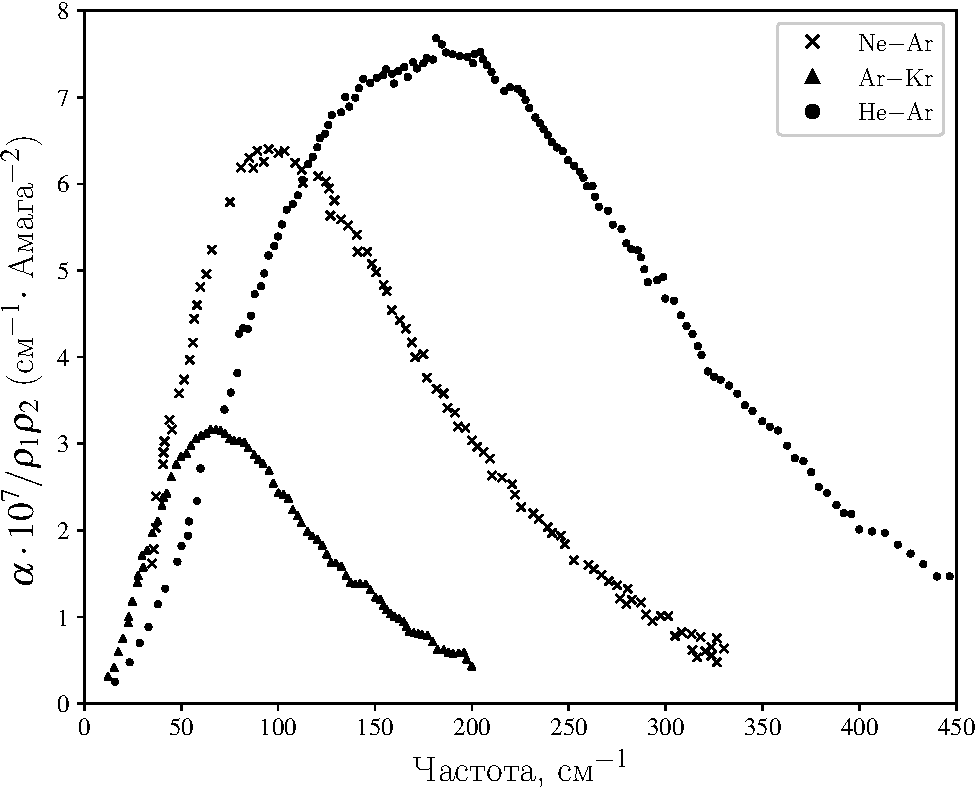
\includegraphics[width=0.7\linewidth]{./pictures/twoatom_experiment/experiment_diatom_spectra-crop.pdf}
    \caption{Экспериментальные спектры бинарного поглощения систем гелий$-$аргон, неон$-$аргон и аргон$-$криптон при комнатной температуре \cite{frommhold}}
    \label{fig:pic-two-atom-experiment}
\end{figure}

В работе \cite{kranendonk1973} авторы разрабатывают формализм расчета столкновительно-индуци\-рован\-ного спектра в приближении бинарных столкновений. Авторы рассматривают систему, состояющую из молекулы H$_2$, взаимодействующей с атомами Ar. Вращательное движение молекулы H$_2$ исключено из рассмотрения -- обе сталкивающихся молекулы рассматриваются как бесструктурные сферически-симметричные частицы. \par
Спектральная функция, определяющая профиль спектра поглощения, связана с функцией автокорреляции суммарного дипольного момента системы преобразованием Фурье \eqref{litreview-spectral-function}. В приближении бинарных столкновений корреляционная функция суммарного дипольного момента принимает вид 
\begin{gather}
    \mean{ \bs{\mu}(0) \bs{\mu}(t) } = N \mean{ \bs{\mu}_1(0) \bs{\mu}_1(t) },
\end{gather} 
%
где через $\bs{\mu_1}(t)$ обозначен дипольный момент, индуцированный квадрупольным полем молекулы H$_2$ на атоме Ar, а $N$ -- количество рассматриваемых пар. Приведенную массу системы авторы обозначают через $\mu$; вектор, соединяющий центр масс молекулы H$_2$ c атомом Ar, -- через $\mathbf{R}$; потенциал взаимодействия -- через $V(R)$ (т.к. вращательное движение молекулы водорода не рассматривается, потенциал зависит только от расстояния между центрами масс $R$). Автокорреляционную функцию дипольного момента приводят к виду 
\begin{gather}
    C(\tau) = \frac{1}{2 \pi} \frac{N}{4 \pi \varepsilon_0} \lb \frac{\mu}{2 \pi k T} \rb^{3/2} \iint \bs{\mu}_1(\mathbf{R}(0)) \cdot \bs{\mu}_1(\mathbf{R}(\tau)) \exp \lb -\frac{\mu \dot{\mf{R}}^2}{2 k T} \rb \zeta(R) \, d \mathbf{R} \, d \dot{\mathbf{R}}, \label{kranendonk-correlation-function}
\end{gather}
%
где $\mathbf{R}(\tau)$ -- значение $\mathbf{R}$, вычисленное в момент времени $\tau$ путем расчета классической траектории, начальными условиями для которой взяты $\mf{R}(0)$ и $\dot{\mf{R}}(0)$, и $\zeta(R)$ -- парная функция распределения 
\begin{gather}
    \zeta(R) = \exp \lb -\frac{V(R)}{kT} \rb.
\end{gather}

Выражение \eqref{kranendonk-correlation-function} неудобно для численного расчета из-за наличия $R(\tau)$ для произвольного момента времени $\tau$. Для более эффективной вычислительной схемы авторы \cite{kranendonk1973} представляют интегральное выражение \eqref{kranendonk-correlation-function} в виде интеграла по полным столкновительным траекториям. При этом будут рассматриваться только траектории рассеяния, связанные состояния исключаются из рассмотрения. В лабораторной системе отсчета энергия система может быть записана в виде
\begin{gather}
    E = \frac{1}{2} \mu \dot{\mf{R}}^2 + V(R).
\end{gather}
Траектория рассеяния, имеющая в момент времени $t$ радиус-вектор $\mf{R}$ и скорость $\dot{\mf{R}}$, однозначно определена относительной скоростью $\mf{g}$ в момент времени $t = -\infty$, прицельным параметром $b$, углом $\varepsilon$, определяющим ориентацию плоскости столковения, и моментом времени $t_0$, в который произошло столкновение. Применяя теорему Лиувилля
\begin{gather}
    d \mf{R} \, d\dot{\mf{R}} = d(t - t_0) b db \, d\varepsilon \, g d\mf{g},
\end{gather}
%
выражение \eqref{kranendonk-correlation-function} преобразуют к виду
\begin{gather}
    C(\tau) = \frac{1}{2 \pi} \frac{N}{4 \pi \varepsilon_0} \lb \frac{\mu}{2 \pi k T} \rb^{3/2} \idotsint \bs{\mu}_1(t) \cdot \bs{\mu}_1(t + \tau) \, \exp \lb - \frac{\mu \mf{g}^2}{2 k T} \rb b \, db \, d\varepsilon \, g d \mf{g} \, dt, \label{correlation-function-kranendonk}
\end{gather}
%
где через $g$ обозначен модуль вектора относительной скорости $\mf{g}$. Используя теорему Винера-Хинчина \cite{frommhold}, авторы \cite{kranendonk1973} получают следующее выражение для спектральной функции 
\begin{gather}
    VJ(\omega) = \frac{1}{2 \pi} \frac{N}{4\pi \varepsilon_0} \lb \frac{\mu}{2 \pi k T} \rb^{3/2} \idotsint \Bigg\vert \intty \bs{\mu}_1(t) e^{-i \omega t} dt \Bigg\vert^2 \, \exp \lb -\frac{\mu g^2}{2 k T} \rb b \, db \, d \varepsilon \, 4 \pi g^3 dg. \label{spectral-function-kranendonk}
\end{gather}

Рассмотрим переход от \eqref{correlation-function-kranendonk} к \eqref{spectral-function-kranendonk} подробно, т.к. мы произведем аналогичное преобразование при выводе альтернативного выражения для спектральной функции в пункте (\ref{section:spectral_function_in_plane}). \par
Корреляцией двух функций $f(z)$ и $g(z)$, определенных на комплексной плоскости $\mathbb{C}$, называют функцию, определенную следующим интегралом
\begin{gather}
    K(z) = \intty f^*(s) g(z + s) ds,
\end{gather}
% 
где $*$ обозначает комплексное сопряжение. Здесь происходит неудачное совпадение названий, т.к. два разных, но близких объекта носят название корреляции. \enquote{Математическую} корреляционную функцию будем обозначать через $K$, а за физическим объектом сохраним обозначение $C$. Обозначим через $F(\omega)$, $G(\omega)$ Фурье-образы функций $f(z)$, $g(z)$. Перепишем выражение для \enquote{математической} корреляции, представив функции через обратное преобразование Фурье от $F(\omega)$, $G(\omega)$, соответственно
\begin{gather}
    K(z) = \intty \lsq \, \intty F^*(\omega) e^{-i \omega s} \frac{d \omega}{2 \pi} \rsq \lsq \, \intty G(\omega^\prime) e^{i \omega^\prime (z + s)} \frac{d\omega^\prime}{2 \pi} \rsq ds.
\end{gather}

Осуществляя перестановку внутри интегрального выражения, приходим к следующему выражению 
\begin{gather}
    K(z) = \frac{1}{2\pi} \intty \intty F^*(\omega) G(\omega^\prime) e^{i \omega^\prime z} \lsq \, \intty e^{i (\omega^\prime - \omega) s} \frac{ds}{2 \pi} \rsq d\omega d\omega^\prime = \notag \\
    = \frac{1}{2\pi} \intty \intty F^*(\omega) G(\omega^\prime) e^{i \omega^\prime z} \delta \lb \omega^\prime - \omega \rb d\omega d\omega^\prime = \hat{F}^{-1} \Big[ F^*(\omega) G(\omega) \Big],
\end{gather}
%
где через $\hat{F}$ обозначен оператор преобразования Фурье. Полученное соотношение, записанное в отношении автокорреляционной функции действительной функции $f$, носит название теоремы Винера-Хинчина \cite{frommhold}
\begin{gather}
    \hat{F} \Big[ K(z) \Big] = \Bigg\vert \hat{F}\Big[ f \Big](\omega) \Bigg\vert^2. 
\end{gather}

Автокорреляционная функция дипольного момента $K(t)$ в подынтегральном выражении \eqref{correlation-function-kranendonk} распадается на сумму автокорреляционных функций $K_\alpha(t)$ компонент дипольного момента 
\begin{gather}
    K(\tau) = \intty \bs{\mu}_1(t) \bs{\mu}_1(t + \tau) dt = \sum_{\alpha = x, y, z} \intty \mu_1^\alpha(t) \mu_1^\alpha(t + \tau) dt = K_x(\tau) + K_y(\tau) + K_z(\tau).
\end{gather}

Следовательно, согласно теореме Винера-Хинчина преобразование Фурье от автокорреляционной функции $K(\tau)$ представляет собой сумму квадратов преобразований Фурье от компонент дипольного момента 
\begin{gather}
    \hat{F}\Big[ K(\tau) \Big] = \sum_{\alpha = x,y,z} \hat{F} \Big[ K_\alpha(\tau) \Big] = \sum_{\alpha=x,y,z} \Bigg\vert \intty \mu_1^\alpha(t) e^{-i\omega t} dt \Bigg\vert^2,
\end{gather}
% 
что для краткости записывают в виде 
\begin{gather}
    \hat{F} \Big[ K(\tau) \Big] = \Bigg\vert \intty \bs{\mu}_1(t) e^{-i\omega t} dt \Bigg\vert^2. \label{correlation-theorem}
\end{gather}

Выражение \eqref{spectral-function-kranendonk} используют при моделировании спектров столкновительно-инду\-ци\-рованного поглощения систем двух атомов методом классических траекторий \cite{levine1967, mcquarrie1968, buryak2014}. Также это выражение можно обобщить на системы, содержащие вращательные степени свободы \cite{oparin2017}. Однако использовать это выражение затруднительно при рассмотрении динамики столкновения в молекулярной системе отсчета, поэтому, используя похожие соображения, мы выведем несколькое иное выражение для спектральной функции для системы двух атомов.

\section{Cистемы координат для описания движения двух атомов} \label{section:two-atom-coordinate-systems}

Рассмотрим движение двух атомов с массами $m_1$, $m_2$ и радиус-векторами $\mf{r}_1$, $\mf{r}_2$ в поле межатомного потенциала $U(\vert \mf{r}_1 - \mf{r}_2 \vert)$. После отделения центра масс задача о движении двух взаимодействующих атомов сводится к задаче о движении виртуальной частицы с приведенной массой $\mu$,  равной 
\begin{gather}
    \mu = \frac{m_1 m_2}{m_1 + m_2}, 
\end{gather}
%
в заданном потенциальном поле $U$ \cite{landau-volume1}. Для описания движения виртуальной частицы введем несколько систем координат. Системой I будем называть декартову систему координат -- положение частицы задается вектором $\mf{r} = \mf{r}_1 - \mf{r}_2$. В этой системе координат лагранжиан и гамильтониан системы записываются как 
\begin{gather}
    \mL_\text{cartesian} = \frac{\mu \dot{\mf{r}}^2}{2} - U( \vert \mf{r} \vert ), \label{two-atom-cartesian-lagrangian} \\
    \mH_\text{cartesian} = \frac{\mf{p}^2}{2\mu} + U( \vert \mf{r} \vert ), \label{two-atom-cartesian-hamiltonian}
\end{gather}
%
где вектор импульса $\mf{p}$ равен
\begin{gather}
    \mf{p} = \frac{\partial \mL_\text{cartesian}}{\partial \dot{\mf{r}}} = \mu \, \dot{\mf{r}}. \label{two-atom-cartesian-momenta}
\end{gather}

Вектор $\mf{r}$ можно представить в сферической системе координат -- длину вектора обозначим через $r$, зенитный и азимутальный углы через $\theta$ и $\varphi$, соответственно ($\theta \in [0, \pi], \varphi \in [0, 2 \pi]$). Будем называть эту координатную систему системой II. Декартовы координаты виртуальной частицы связаны со сферическими координатами следующими соотношениями
\begin{gather}
    \lc
    \begin{aligned}
        x &= r \cos \varphi \sin \theta \\
        y &= r \sin \varphi \sin \theta \\
        z &= r \cos \theta
    \end{aligned}
    \right. \label{two-atom-spherical-coordinates}
\end{gather}

Лагранжиан и гамильтониан в системе координат II записываются как
\begin{gather}
    \mL_\text{spherical} = \frac{1}{2} \mu \dot{r}^2 + \frac{1}{2} \mu r^2 \dot{\theta}^2 + \frac{1}{2} \mu r^2 \dot{\varphi}^2 \sin^2 \theta - U(r),  \label{two-atom-spherical-lagrangian} \\
    \mH_\text{spherical} = \frac{p_r^2}{2 \mu} + \frac{p_\theta^2}{2 \mu r^2} + \frac{p_\varphi^2}{2 \mu r^2 \sin^2 \theta} + U(r), \label{two-atom-spherical-hamiltonian}
\end{gather}
%
где обобщенные импульсы $p_r$, $p_\theta$, $p_\varphi$ связаны с обобщенными скоростями соотношениями
\begin{gather}
    p_r = \frac{\partial \mL_\text{spherical}}{\partial \dot{r}} = \mu \dot{r} \quad \Longrightarrow \quad \dot{r} = \frac{p_r}{\mu}, \label{two-atom-spherical-momenta1} \\
    p_\theta = \frac{\partial \mL_\text{spherical}}{\partial \dot{\theta}} = \mu r^2 \dot{\theta} \quad \Longrightarrow \quad \dot{\theta} = \frac{p_\theta}{\mu r^2}, \label{two-atom-spherical-momenta2} \\
    p_\varphi = \frac{\partial \mL_\text{spherical}}{\partial \dot{\varphi}} = \mu r^2 \dot{\varphi} \sin^2 \theta \quad \Longrightarrow \quad \dot{\varphi} = \frac{p_\varphi}{\mu r^2 \sin^2 \theta}. \label{two-atom-spherical-momenta3}
\end{gather}

Рассмотрим, как связаны декартовы импульсы $\mf{p}$ с импульсами $p_r$, $p_\theta$, $p_\varphi$, сопряженными сферическим координатам. Для этого продифференцируем соотношения \eqref{two-atom-spherical-coordinates} по времени и умножим обе части на приведенную массу $\mu$. Получим в левой части компоненты вектора $\mf{p}$ (согласно \eqref{two-atom-cartesian-momenta}), а в правой части подставим выражения обобщенных скоростей $\dot{r}$, $\dot{\theta}$, $\dot{\varphi}$ через соответствующие импульсы \eqref{two-atom-spherical-momenta1}, \eqref{two-atom-spherical-momenta2}, \eqref{two-atom-spherical-momenta3}
\begin{gather}
    \lc 
    \begin{aligned}
        p_x &= p_r \cos \varphi \sin \theta + \frac{p_\theta}{r} \cos \varphi \cos \theta - \frac{p_\varphi}{r} \frac{\sin \varphi}{\sin \theta}, \\ 
        p_y &= p_r \sin \varphi \sin \theta + \frac{p_\theta}{r} \sin \varphi \cos \theta + \frac{p_\varphi}{r} \frac{\cos \varphi}{\sin \theta}, \\ 
        p_z &= p_r \cos \theta - \frac{p_\theta}{r} \sin \theta.
    \end{aligned}
    \right. \label{two-atom-cartesian-spherical-momenta}
\end{gather}

Разрешая линейные соотношения \eqref{two-atom-cartesian-spherical-momenta} относительно импульсов $p_r$, $p_\theta$, $p_\varphi$, находим соотношения, выражающие обратную связь импульсов
\begin{gather}
    \lc
    \begin{aligned}
        p_r &= r \lb p_x \cos \varphi \sin \theta + p_y \sin \varphi \sin \theta + p_z \cos \theta \rb, \\
        p_\varphi &= r \sin \theta \lb p_y \cos \varphi - p_x \sin \varphi \rb, \\
        p_\theta &= r \lb p_x \cos \varphi \cos \theta + p_y \sin \varphi \cos \theta - p_z \sin \theta \rb.  
    \end{aligned}
    \right.
\end{gather}

Выразим компоненты углового момента через координаты и импульсы системы II, пользуясь соотношениями \eqref{two-atom-cartesian-spherical-momenta}
\begin{gather}
    \mf{J} = \lsq \mf{r} \times \mf{p} \rsq = 
    \begin{bmatrix}
        -p_\theta \sin \varphi - p_\varphi \cos \varphi \cot \theta \\
        -p_\varphi \sin \varphi \cot \theta + p_\theta \cos \varphi \\
        p_\varphi
    \end{bmatrix}. \label{two-atom-angular-momenta-spherical} 
\end{gather}

Известно, что в отсутствии внешнего момента сил угловой момент является векторным интегралом движения, следовательно движение двух атомов происходит в перпендикулярной ему плоскости \cite{goldstein}. Для описания динамики системы введем полярные координаты $r, \psi$ и соответствующие обобщенные скорости $\dot{r}$, $\dot{\psi}$. Ориентацию плоскости будем задавать при помощи пары сферических углов $\Phi$, $\Theta$, описывающих направление вектора углового момента. Определим систему координат таким образом, чтобы координатная плоскость $OXY$ совпадала с плоскостью движения, а ось $OZ$ была сонаправлена с вектором углового момента $\mf{J}$. Будет называть эту координатную систему системой III; лагранжиан и гамильтониан в ней равны 
\begin{gather}
    \mL_\text{plane} = \frac{1}{2} \mu \dot{r}^2 + \frac{1}{2} \mu r^2 \dot{\psi}^2 - U(r), \label{two-atom-plane-lagrangian} \\
    \mH_\text{plane} = \frac{p_r^2}{2\mu} + \frac{p_\psi^2}{2 \mu r^2} + U(r), \label{two-atom-plane-hamiltonian} 
\end{gather}
%
где обобщенные импульсы $p_r$, $p_\psi$ связаны с обобщенными скоростями следующими соотношениями
\begin{gather}
    p_r = \frac{\partial \mL_\text{plane}}{\partial \dot{r}} = \mu \dot{r} \quad \Longrightarrow \quad \dot{r} = \frac{p_r}{\mu}, \label{two-atom-plane-momenta1} \\
    p_\psi = \frac{\partial \mL_\text{plane}}{\partial \dot{\psi}} = \mu r^2 \dot{\psi} \quad \Longrightarrow \quad \dot{\psi} = \frac{p_\psi}{\mu r^2}.  \label{two-atom-plane-momenta2}
\end{gather}

Перевод полярных координат $r$, $\psi$ системы III в декартовы координаты $\mf{r} = \lc x, y, z \rc$ системы I можно осуществить при помощи ортогональной матрицы вращения $\bbS$, параметризованной углами $\Phi$, $\Theta$ \cite{goldstein} 
\begin{gather}
    \begin{bmatrix}
        x \\ y \\ z
    \end{bmatrix} 
    = \bbS_\Phi^{-1} \bbS_\Theta^{-1} 
    \begin{bmatrix}
        r \cos \psi \\ r \sin \psi \\ 0
    \end{bmatrix}, \label{two-atoms-coordinate-transformation}
\end{gather}
% 
где матрицы поворота $\bbS_\Phi$, $\bbS_\Theta$ равны
\begin{gather}
    \bbS_\Phi = 
    \begin{bmatrix}
       -\sin \Phi & \cos \Phi & 0 \\
       -\cos \Phi & -\sin \Phi & 0 \\
      0 & 0 & 1
    \end{bmatrix}, \quad
    \bbS_\Theta = 
    \begin{bmatrix}
        1 & 0 & 0 \\
        0 & \cos \Theta & \sin \Theta \\
        0 & -\sin \Theta & \cos \Theta
    \end{bmatrix}.
\end{gather}

Раскрывая матричное выражение \eqref{two-atoms-coordinate-transformation}, получаем 
\begin{gather}
    \left\{
        \begin{aligned}
            x &= -r \cos \psi \sin \Phi - r \sin \psi \cos \Phi \cos \Theta \\
            y &= r \cos \psi \cos \Phi - r \sin \psi \sin \Phi \cos \Theta \\
            z &= r \sin \psi \sin \Theta
        \end{aligned}
    \right. \label{two-atoms-coordinates-transformation2}
\end{gather}

Продифференцируем соотношения \eqref{two-atoms-coordinates-transformation2} по времени, учитывая, что углы $\Phi$, $\Theta$ от времени не зависят.
\begin{gather}
    \begin{bmatrix} \dot{x} \\ \dot{y} \\ \dot{z} \end{bmatrix} = 
    \bbS_\Phi^{-1} \bbS_\Theta^{-1}
    \begin{bmatrix} 
        \dot{r} \cos \psi - r \dot{\psi} \sin \psi \\
        \dot{r} \sin \psi + r \dot{\psi} \cos \psi \\
        0 
    \end{bmatrix} \\
    \lc
    \begin{aligned}
        \dot{x} &= - \dot{r} \lb \cos \psi \sin \Phi + \sin \psi \cos \Phi \cos \Theta \rb + r \dot{\psi} \lb \sin \psi \sin \Phi - \cos \psi \cos \Phi \cos \Theta \rb \\ 
        \dot{y} &= \dot{r} \lb \cos \psi \cos \Phi - \sin \psi \sin \Phi \sin \Theta \rb - r \dot{\psi} \lb \sin \psi \cos \Phi - \cos \psi \sin \Phi \cos \Theta \rb \\
        \dot{z} &= \dot{r} \sin \psi \sin \Theta + r \dot{\psi} \cos \psi \sin \Theta
    \end{aligned}
\right. \label{two-atoms-coordinates-transformation3}
\end{gather}

При рассмотрении средних значений функций по фазовому пространству нам понадобятся выражения импульсов $\mf{p}$ через импульсы $p_r$, $p_\psi$. При умножении левых частей соотношений \eqref{two-atoms-coordinates-transformation3} на приведенную массу $\mu$ мы получим компоненты вектора $\mf{p}$ (согласно \eqref{two-atom-cartesian-momenta}). Подставив выражения обобщенных скоростей $\dot{r}$, $\dot{\psi}$ через импульсы $p_r$, $p_\psi$ (\eqref{two-atom-plane-momenta1}, \eqref{two-atom-plane-momenta2}), получаем
\begin{gather}
    \lc
    \begin{aligned}
        p_x &= -p_r \lb \sin \psi \cos \Phi \cos \Theta + \cos \psi \sin \Phi \rb + \frac{p_\psi}{r} \lb \sin \psi \sin \Phi - \cos \psi \cos \Phi \cos \Theta \rb \\
        p_y &= p_r \lb \cos \psi \cos \Phi - \sin \psi \sin \Phi \cos \Theta \rb - \frac{p_\psi}{r} \lb \sin \psi \cos \Phi + \cos \psi \sin \Phi \cos \Theta \rb \\
        p_z &= p_r \sin \psi \sin \Theta + \frac{p_\psi}{r} \cos \psi \sin \Theta 
    \end{aligned}
\right. \label{two-atom-momenta-transformation}
\end{gather}

Выразим компоненты углового момента через координаты системы III, исходя из определения вектора углового момента 
\begin{gather}
    \mf{J} = \mu \lsq \mf{r} \times \dot{\mf{r}} \rsq = 
    \begin{bmatrix}
        \mu r^2 \dot{\psi} \cos \Phi \sin \Theta \\ 
        \mu r^2 \dot{\psi} \sin \Phi \sin \Theta \\
        \mu r^2 \dot{\psi} \cos \Theta
    \end{bmatrix},
\end{gather}
или, пользуясь соотношением между скоростью $\dot{\psi}$ и импульсом $p_\psi$ \eqref{two-atom-plane-momenta2}, 
\begin{gather}
    \mf{J} = 
    \begin{bmatrix}
        p_\psi \cos \Phi \sin \Theta \\
        p_\psi \sin \Phi \sin \Theta \\
        p_\psi \cos \Theta
    \end{bmatrix}. \label{two-atom-plane-angular-momenta}
\end{gather}

Выражение \eqref{two-atom-plane-angular-momenta} показывает, что углы $\Phi$, $\Theta$ являются сферическими углами для вектора углового момента. Кроме того, замечаем, что импульс $p_\psi$ имеет физический смысл модуля вектора углового момента. 

\section{Усреднение функций по фазовому пространству в разных системах координат} \label{section:averaging}

Рассмотрим усреднение некоторой функции $f(\mf{r}, \mf{p})$ по фазовому пространству двухатомной системы, где $\mf{r}$, $\mf{p}$ -- векторы декартовых координат и сопряженных импульсов (система I): 
\begin{gather}
    \mean{f} = \idotsint f(\mf{r}, \mf{p}) \exp \lb -\frac{\mH(\mf{r},\mf{p})}{kT} \rb d \mf{r} \, d\mf{p}. \label{two-atom-mean}
\end{gather}

Целью нашего рассмотрения будет отыскание выражений, позволяющих производить усреднение функции $f$ по фазовому пространству, пользуясь координатами систем II и III. \par
Рассмотрим совокупную систему уравнений \eqref{two-atoms-coordinates-transformation2}, \eqref{two-atom-momenta-transformation} и найдем якобиан замены переменных $\lc x, y, z, p_x, p_y, p_z \rc$ $\rightarrow$ $\lc r, p_r, \psi, p_\psi, \Phi, \Theta \rc$. Ввиду громоздкости выкладки приводить не будем, выражение для якобиана получается следующее:
\begin{gather}
    \text{Jac} = \Bigg\vert \frac{\partial \lsq x, y, z, p_x, p_y, p_z \rsq}{\partial \lsq r, p_r, \psi, p_\psi, \Phi, \Theta \rsq} \Bigg\vert = p_\psi \sin \Theta. \label{two-atom-planar-jacobian}
\end{gather}

Итак, среднее значение \eqref{two-atom-mean} в системе координат III записывается как
\begin{gather}
    \mean{ f } = \int\limits_{0}^{\infty} dr \intty dp_r \int\limits_0^{2\pi} d\psi \int\limits_0^\infty p_\psi dp_\psi \int\limits_0^\pi \sin \Theta d\Theta \int\limits_0^{2\pi} d\Phi f(r, \psi, p_r, p_\psi, \Theta, \Phi) \exp \lb -\frac{\mH_\text{plane}}{k T} \rb. \label{two-atom-mean-plane1} 
\end{gather}

Если усредняемая функция $f(r, \psi, p_r, p_\psi, \Theta, \Phi)$ не зависит от углов $\Theta$, $\Phi$, то среднее значение  \eqref{two-atom-mean-plane1} принимает вид 
\begin{gather}
    \mean{ f } = 4 \pi \int\limits_{0}^{\infty} dr \intty dp_r \int\limits_0^{2\pi} d\psi \int\limits_0^\infty p_\psi dp_\psi f(r, \psi, p_r, p_\psi, \Theta, \Phi) \exp \lb -\frac{\mH_\text{plane}}{k T} \rb. \label{two-atom-mean-plane2} 
\end{gather}

Как уже отмечалось ранее, импульс $p_\psi$ имеет физический смысл модуля углового момента, поэтому область интегрирования этого импульса составляет полуось $(0, +\infty)$, в то время как для радиального импульса -- вся прямая $(-\infty, +\infty)$. \par
Аналогично, рассмотрим совокупную систему уравнений \eqref{two-atom-spherical-coordinates}, \eqref{two-atom-cartesian-spherical-momenta} и найдем якобиан замены переменных $\lc x, y, z, p_x, p_y, p_z \rc$ $\rightarrow$ $\lc r, p_r, \varphi, p_\varphi, \theta, p_\theta \rc$. Якобиан оказывается единичным: 
\begin{gather}
    \text{Jac} = \Bigg\vert \frac{\partial \lsq x, y, z, p_x, p_y, p_z \rsq}{\partial \lsq r, p_r, \varphi, p_\varphi, \theta, p_\theta \rsq} \Bigg\vert = 1. 
\end{gather}

Таким образом, среднее значение \eqref{two-atom-mean} в системе координат II записывается как
\begin{gather}
    \mean{f} = \int\limits_0^\infty dr \intty dp_r \int\limits_0^{2\pi} d\varphi \intty dp_\varphi \int\limits_0^\pi d\theta \intty dp_\theta f(r, p_r, \varphi, p_\varphi, \theta, p_\theta) \exp \lb -\frac{\mH_\text{spherical}}{k T} \rb. \label{two-atom-mean-spherical}
\end{gather}

\section{Распределения координат и импульсов в фазовом пространстве в разных системах координат} \label{section:two-atom-distributions} 

Рассмотрим вопрос распределения координат и импульсов в фазовом пространстве в системах координат II и III в условиях канонического ансамбля. Функция распределения в фазовом пространстве в условиях канонического ансамбля задана гамильтонианом системы $\mH$ \cite{hill} 
\begin{gather}
    \rho \lb \mf{q}, \mf{p} \rb = \Gamma_0 \exp \lb -\frac{\mH \lb \mf{q}, \mf{p} \rb}{\kb T} \rb,
\end{gather}
% 
где постоянная $\Gamma_0$ определяется из условия нормировки функции распределения
\begin{gather}
    \int \rho \lb \mf{q}, \mf{p} \rb d \mf{q} \, d\mf{p} = 1.
\end{gather}

Рассмотрим распределения угловых координат $\theta, \varphi$ и импульсов $p_r$, $p_\theta$, $p_\varphi$ системы II при фиксированном большом значении межатомного расстояния $r_\text{fixed} \gg 1$. Пренебрежем значением потенциала $U(r_\text{fixed}) \approx 0$ на расстоянии $r_\text{fixed}$ (для системы He$-$Ar было использовано фиксированное межатомное расстояние, равное $\rfixed = 40 a_0$, где через $a_0$ обозначен Боровский радиус). Удобно представить отношение $\mH / \kb T$ в виде трех квадратичных членов $\lc \frac{1}{2} x_j^2 \rc_{j = 1 \dots 3}$
\begin{gather}
    \frac{\mH_\text{spherical}}{\kb T} = \frac{p_r^2}{2 \mu \kb T} + \frac{p_\theta^2}{2 \mu r_\text{fixed}^2 \kb T} + \frac{p_\varphi^2}{2 \mu r_\text{fixed}^2 \kb T \sin^2 \theta} = \frac{1}{2} x_1^2 + \frac{1}{2} x_2^2 + \frac{1}{2} x_3^2, \label{two-atom-spherical-hamiltonian-xs} 
\end{gather}
%
где переменные $x_j$ выражены как
\begin{gather}
    \lc
    \begin{aligned}
        x_1 &= \frac{p_r}{\sqrt{\mu \kb T}}, \\
        x_2 &= \frac{p_\theta}{\sqrt{\mu r_\text{fixed}^2 \kb T}}, \\
        x_3 &= \frac{p_\varphi}{\sqrt{\mu r_\text{fixed}^2 \kb T \sin^2 \theta}}.
    \end{aligned}
\right. \label{two-atom-xs}
\end{gather}

Переписав гамильтониан в виде \eqref{two-atom-spherical-hamiltonian-xs}, мы видим, что вероятность нахождения системы в элементе фазового объема $d\theta d\varphi dx_1 dx_2 dx_3$ пропорциональна произведению 
\begin{gather}
    \rho \lb \theta, \varphi, x_1, x_2, x_3 \rb \propto \rho_1(x_1) \rho_1(x_2) \rho_1(x_3) \sin \theta, \label{two-atom-xs-phase-element}
\end{gather}
%
где случайные величины $x_j$ распределены по нормальному закону
\begin{gather}
    \rho_1 (x_j) = \frac{1}{\sqrt{2 \pi}} \exp \lb -\frac{x_j^2}{2} \rb. 
\end{gather}

Соотношения \eqref{two-atom-xs} позволяют установить следующие функции распределения для двух импульсов
\begin{gather}
    \lc
    \begin{aligned}
        p_r &\sim \mN \lb 0, \mu \kb T \rb, \\
        p_\theta &\sim \mN \lb 0, \mu r_\text{fixed}^2 \kb T \rb, 
    \end{aligned}
    \right.
\end{gather}
%
где через $\mN \lb \mu, \sigma^2 \rb$ обозначено нормальное распределение с математическим ожиданием $\mu$ и дисперсией $\sigma^2$. Импульс $p_\varphi$ представляет собой произведение двух случайных величин
\begin{gather}
    p_\varphi = x_3 \cdot \sin \Theta, \label{two-atom-pvarphi-generation}
\end{gather}
% 
где величина $x_3$ распределена по нормальному закону $\mN \lb 0, \mu r_\text{fixed}^2 \kb T \rb$, а плотность распределения случайной величины $\Theta$ в силу \eqref{two-atom-xs-phase-element} равна
\begin{gather}
    \rho(\Theta) = \frac{1}{2} \sin \Theta.
\end{gather}

Численная генерация случайных величин $p_\varphi$ легко осуществляется по выражению \eqref{two-atom-pvarphi-generation}, однако интересно получить аналитическое выражение для плотности распределения, так как такие же распределения возникают при рассмотрении импульсов в многоатомных комплексах. Сначала получим плотность распределения величины $\sin \Theta$, используя то, что $\cos \Theta$ распределен равномерно на отрезке $\lsq -1, 1\rsq$. Очевидно, что в области определения зенитного угла $\lsq 0, \pi \rsq$ знак $\sin \Theta$ определен однозначно, следовательно выбираем положительный знак корня 
\begin{gather}
    \sin \Theta = \sqrt{ 1 - \cos^2 \Theta}.
\end{gather}
Далее воспользуемся формулой преобразования случайной величины $Y = g(X)$
\begin{gather}
    \rho_Y(y) = \Big\vert \frac{d}{dy} g^{-1}(y) \Big\vert \cdot \rho_X(g^{-1}(y)), \label{distribution-change}
\end{gather}
%
где через $\rho_X(x)$, $\rho_Y(y)$ обозначены плотности случайных величин $X$, $Y$, соответственно. В данном случае преобразование осуществляется функцией $g(x) = \sqrt{1 - x^2}$, подстановка которой в \eqref{distribution-change} приводит к следующей плотности распределения для $\sin \Theta$ 
\begin{gather}
    \rho_{\sin \Theta}(x) = \frac{x}{\sqrt{1 - x^2}} \cdot \bbI\lsq 0, 1\rsq,
\end{gather}
% 
где через $\bbI\lsq 0, 1 \rsq$ обозначена индикаторная функция, ограничивающая носитель функции отрезком $\lsq 0, 1 \rsq$. Отметим, что полученное распределение является частным случаем распределения Кумарасвами с параметрами $a = 2$, $b = 1/2$ \cite{kumaraswamy1980}. \par
Плотность распределения $\rho_{p_\varphi}$ может быть получена по стандартной формуле плотности случайной величины, являющейся произведением двух других случайных величин
\begin{gather}
    \rho_{p_\varphi}(z) = \intty \rho_{x_3}(z/x) \rho_{\sin \Theta}(x) \frac{dx}{\vert x \vert}.
\end{gather}
Подставив явные выражения для плотностей распределения, получаем следующий интеграл
\begin{gather}
    \rho_{p_\varphi}(z) = \frac{1}{\sqrt{2 \pi}} \int\limits_0^1 \frac{\displaystyle \exp \lb -\frac{z^2}{2x^2} \rb}{\sqrt{1 - x^2}} dx,
\end{gather}
%
разрешив который приходим к
\begin{gather}
    \rho_{p_\varphi}(z) = \frac{\pi}{8} \lb 1 - \text{sgn}(z) \text{erf} \lb \frac{z}{\sqrt{2}} \rb \rb.
\end{gather}
Так как угол $\varphi$ не входит в гамильтониан $\mH_\text{spherical}$, то он распределен с равномерной плотностью на отрезке $\lsq 0, 2 \pi \rsq$.

\setcounter{figure}{1}
\begin{figure}[H]
    \centering
    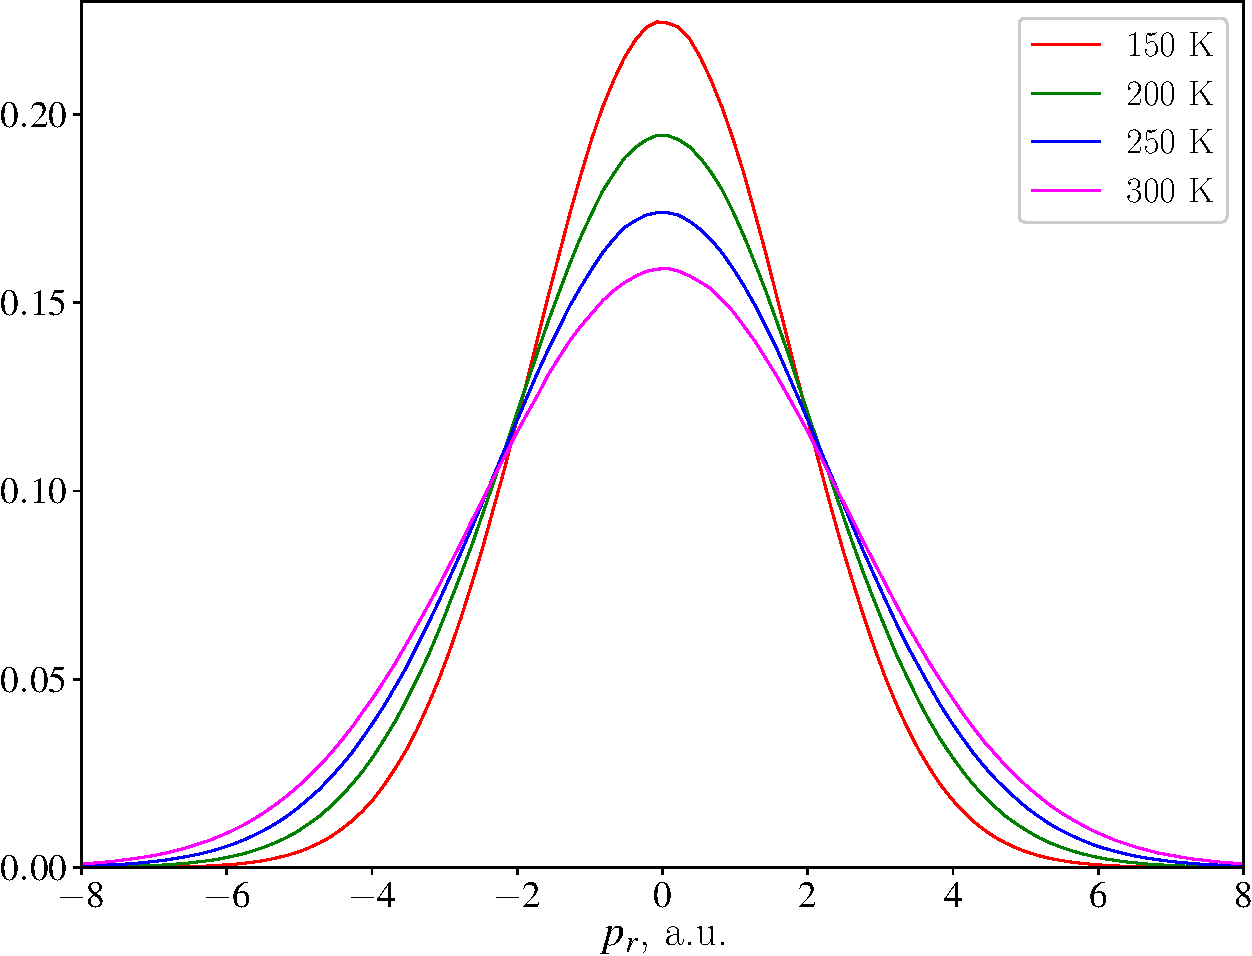
\includegraphics[width=0.75\linewidth]{./pictures/two_atom_distributions/pR-crop.pdf} \\
    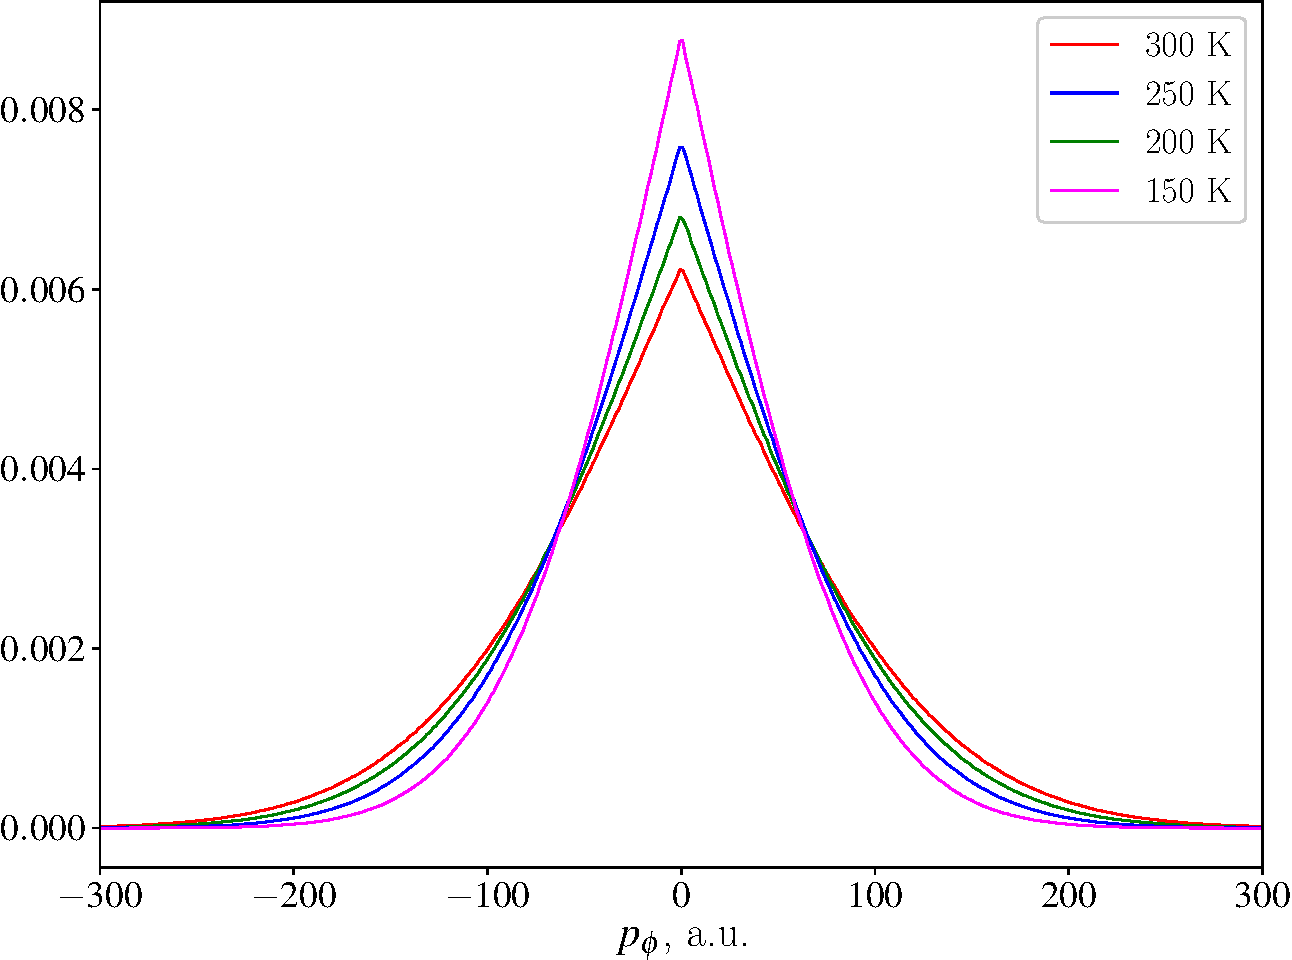
\includegraphics[width=0.75\linewidth]{./pictures/two_atom_distributions/pPhi-crop.pdf}
    \caption{Плотности распределений импульсов $p_r$ и $p_\varphi$ при температурах от 150K до 300K с шагом 50K для системы He$-$Ar. Максимумы плотностей распределений убывают с увеличением температуры. Межатомное расстояние $r_\text{fixed}$ взято равным $40 a_0$. Количество сгенерированных точек при каждой температуре -- $N = 5 \cdot 10^7$.}
    \label{fig:pr-pphi-distributions}
\end{figure}

Если переходить теперь к переменным системы координат III, то легко заметить, что плотность распределения импульса $p_r$ совпадает с той, что была получена в системе координат II. Угол $\psi$ не входит в гамильтониан, следовательно распределен с равномерной плотностью. Так как якобиан замены декартовых координат и импульсов на координаты и импульсы системы III равен $p_\psi \sin \Theta$ (соотношение \eqref{two-atom-planar-jacobian}), то получаем, что плотность распределения импульса $p_\psi$ пропорциональна
\begin{gather}
    \rho(p_\psi) \propto p_\psi \exp \lb -\frac{p_\psi^2}{2 \mu r_\text{fixed}^2 \kb T} \rb, \label{two-atom-ppsi-distribution}
\end{gather}
где коэффициент пропорциональности устанавливается из условия нормировки и оказывается равным $1/(\mu r_\text{fixed}^2 \kb T)$. Из вида якобиана \eqref{two-atom-planar-jacobian} вытекает, что угол $\Theta$ распределен равномерно с косинусом. \par
Распределение для импульса $p_\psi$ может быть установлено и из других соображений. Как уже отмечалось, $p_\psi$ имеет физический смысл модуля углового момента $\mf{J}$. Исходя из выражения \eqref{two-atom-angular-momenta-spherical}, получаем, что квадрат модуля углового момента $J^2$ связан с импульсами $p_\varphi$, $p_\theta$ соотношением
\begin{gather}
    J^2 = p_\psi^2 = p_\theta^2 + \frac{p_\varphi^2}{\sin^2 \theta}. \label{two-atom-angular-momenta-connection} 
\end{gather}
Мы уже установили, что величины $p_\theta$ и $p_\varphi / \sin \theta$ распределены согласно нормальному закону. Квадраты нормально распределенных случайных величин распределены согласно хи-квадрат распределению с одной степенью свободы $\chi_1^2$ \cite{castaneda}. А сумма двух одномерных хи-квадрат распределений $\chi_1^2$ дает двумерное хи-квадрат распределение $\chi_2^2$. Наконец, для того чтобы получить распределение величины $p_\psi$, извлекаем корень из двумерного хи-квадрат распределения $\chi_2^2$ и получаем двумерное хи-распределение $\chi_2$, известное как распределение Рэлея, плотность которого задается  
\begin{gather}
    \rho(x; \sigma) = \frac{x}{\sigma^2} \exp \lb -\frac{x^2}{2 \sigma^2} \rb. \label{rayleigh-density}
\end{gather}

Выражение \eqref{two-atom-ppsi-distribution} является частным случаем распределением Рэлея с параметром $\sigma^2 = \mu r_\text{fixed}^2 \kb T$.

\setcounter{figure}{2}
\begin{figure}[H]
    \centering
    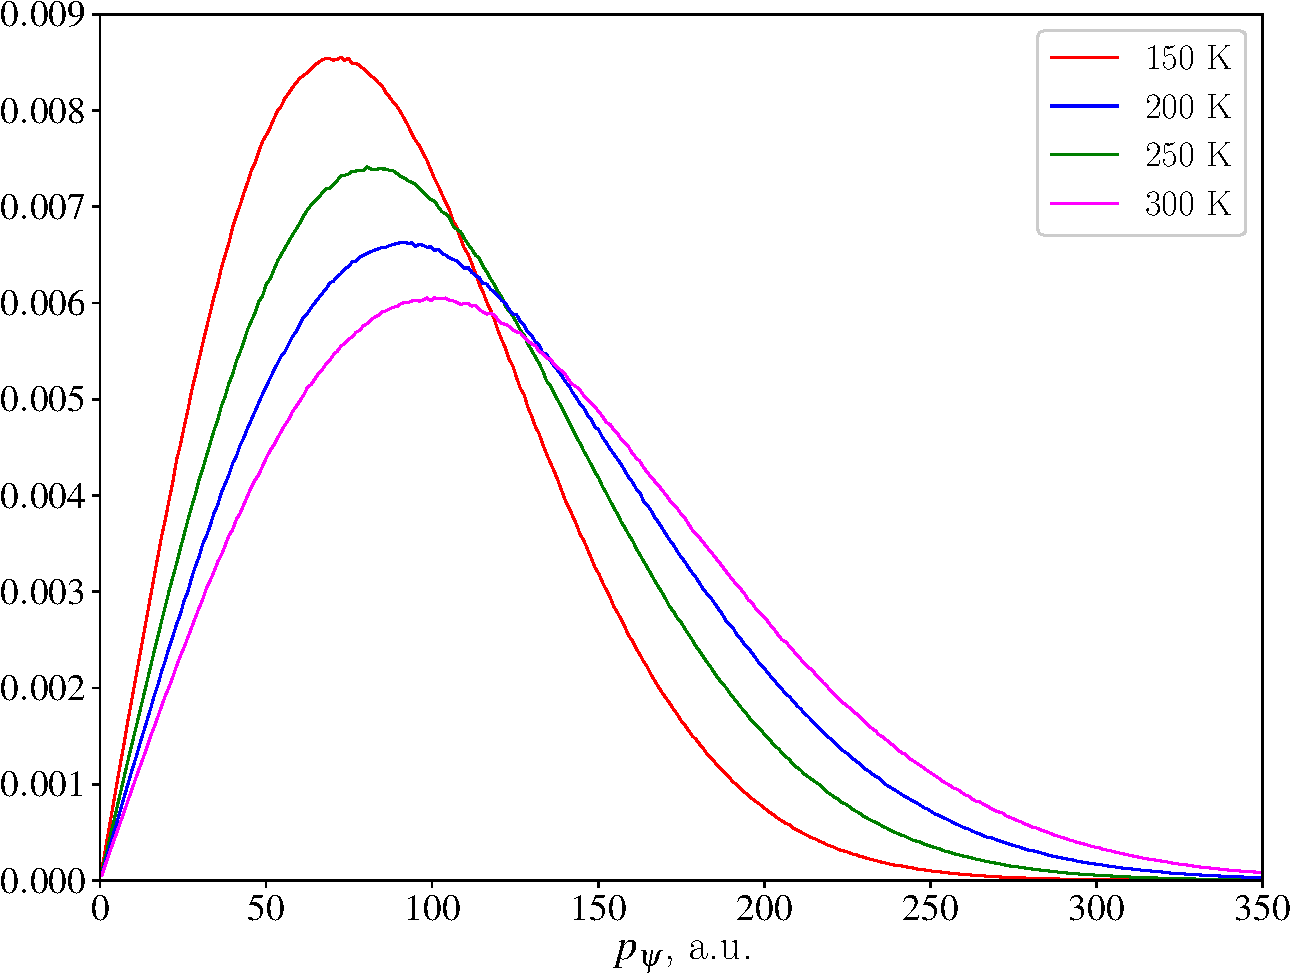
\includegraphics[width=0.75\linewidth]{./pictures/two_atom_distributions/pPsi-crop.pdf}
    \caption{Плотности распределений импульса $p_\psi$ при температурах от 150К до 300К с шагом 50К для системы He$-$Ar. Максимумы распределений уменьшаются и сдвигаются вправо с уменьшением температуры. Межатомное расстояние $r_\text{fixed}$ было взято равным $40a_0$. Количество сгенерированных точек при каждой температуре -- $N = 5 \cdot 10^7$.}
    \label{fig:ppsi-distributions}
\end{figure}

\section{Спектральная функция при рассмотрении динамики столкновения в плоскости} \label{section:spectral_function_in_plane}

Рассмотрим произведение спектральной функции на объем, являющееся преобразованием Фурье от автокорреляционной функции дипольного момента согласно \eqref{litreview-autocorrelation-function-definition}   
\begin{gather}
    VJ(\omega) = \frac{1}{2 \pi} \frac{V}{4 \pi \varepsilon_0} \intty \mean{ \bs{\mu}(0) \bs{\mu}(t) } e^{-i \omega t} dt.
\end{gather}

Мы будем пользоваться приближением бинарных столкновений, то есть будем предполагать, что суммарная автокорреляционная функция распадается на сумму автокорреляционных функций индуцированных диполей пар. Для индуцированного дипольного момента пары мы сохраним для простоты  обозначение $\bs{\mu}$. Итак, мы будем работать со следующим выражением для спектральной функции с трактовкой интеграла как интеграла по начальным условиям классических динамических траекторий, как обсуждалось в пункте \ref{section:correlation_functions} 
\begin{gather}
    VJ(\omega) = \frac{1}{2\pi} \frac{V}{4 \pi \varepsilon_0} \intty \frac{\displaystyle \idotsint \bs{\mu}(0) \bs{\mu}(t) \, \exp \lb -\frac{\mH}{kT} \rb d\mf{q} \, d\mf{p}}{\displaystyle \idotsint \exp \lb -\frac{\mH}{kT} \rb d\mf{q} \, d\mf{p}} e^{-i \omega t} dt. \label{two-atom-spectral-function1}
\end{gather}

Вектор координат при рассмотрении в плоскости столкновений равен $\mf{q} = \lc r, \psi, \Phi, \Theta \rc$, а вектор импульсов -- $\mf{p} = \lc p_r, p_\psi \rc$. Кроме того, согласно пункту \ref{section:averaging} в интеграле появляется дополнительный весовой множитель, равный $\text{Jac} = p_\psi \sin \Theta$. Следовательно, полное интегральное выражение в этой системе координат выглядит следующим образом
\begin{gather}
    VJ(\omega) = \frac{1}{2\pi} \frac{V}{4 \pi \varepsilon_0} \intty e^{-i\omega t} dt \frac{\displaystyle \int\limits_0^\infty dr \intty dp_r \int\limits_0^{2\pi} d\psi \int\limits_0^\infty p_\psi dp_\psi \int\limits_0^\pi \sin \Theta d\Theta \int\limits_0^{2\pi} d\Phi \bs{\mu}(0) \bs{\mu}(t) \exp \lb -\frac{\mH_\text{plane}}{kT} \rb}{\displaystyle \int\limits_0^\infty dr \intty dp_r \int\limits_0^{2\pi} d\psi \int\limits_0^\infty p_\psi dp_\psi \int\limits_0^\pi \sin \Theta d\Theta \int\limits_0^{2\pi} d\Phi \exp \lb -\frac{\mH_\text{plane}}{kT} \rb}. \label{two-atom-spectral-function2}
\end{gather}

Заметим, что скалярное произведение дипольных моментов $\bs{\mu}(0) \bs{\mu}(t)$ и гамильтониан $\mH$ не зависят от углов $\Phi$, $\Theta$. Проинтегрировав по ним, мы получаем множитель $4 \pi$ как в числителе, так и знаменателе, поэтому суммарно никаких дополнительных множителей не возникает.
\begin{gather}
    VJ(\omega) = \frac{1}{2 \pi} \frac{V}{4 \pi \varepsilon_0} \intty e^{-i\omega t} dt \frac{\displaystyle \int\limits_0^\infty dr \intty dp_r \int\limits_0^{2\pi} d\psi \int\limits_0^\infty p_\psi dp_\psi \bs{\mu}(0) \bs{\mu}(t) \exp \lb -\frac{\mH_\text{plane}}{kT} \rb}{\displaystyle \int\limits_0^\infty dr \intty dp_r \int\limits_0^{2\pi} d\psi \int\limits_0^\infty p_\psi dp_\psi \exp \lb -\frac{\mH_\text{plane}}{kT} \rb}. \label{two-atom-spectral-function3}
\end{gather}

Как известно, решение задачи о движении частицы с приведенной массой $\mu$ в центральном поле можно получить, основываясь на законах сохранения энергии и углового момента в интегральном виде \cite{landau-volume1}. Гамильтониан, записанный в полярных координатах, определенных в плоскости движения (система III), 
\begin{gather}
    \mH_\text{plane} = \frac{p_r^2}{2\mu} + \frac{p_\psi^2}{2\mu r^2} + U(r) = E,
\end{gather}
%
является интегралом движения. Импульс $p_\psi$ также является интегралом движения. Решение уравнений движения в интегральном виде выглядит следующим образом \cite{landau-volume1} 
\begin{gather}
    t = \int\limits_{r_\text{нач}}^{r} \frac{dr}{\displaystyle \sqrt{\frac{2}{\mu} \lb E - U(r) \rb - \frac{p_\psi^2}{\mu^2 r^2}}}, \label{two-atom-change1} \\
    \psi = \int\limits_{r_\text{нач}}^{r} \frac{\displaystyle \frac{p_\psi}{r^2} dr}{\displaystyle \sqrt{2\mu \lb E - U(r) \rb - \frac{p_\psi^2}{r^2}}}, \label{two-atom-change2}
\end{gather}
где $r_\text{нач}$ -- начальное значение межатомного расстояния, а $r$ -- межатомное расстояние в момент времени $t$.  

Рассмотрим замену координат в интеграле в числителе \eqref{two-atom-spectral-function3} следующего вида
\begin{gather}
    \lc r, p_r, \psi, p_\psi \rc \rightarrow \lc (\rfixed), \tau, p_r^\prime, \psi^\prime, p_\psi \rc \label{two-atom-change-variables-time}.
\end{gather}

Физический смысл этой замены координат состоит в том, что вместо того чтобы начинать классическую траекторию с произвольного межатомного расстояния $r$, мы хотим использовать фиксированное начальное расстояние $\rfixed$ ($\rfixed$ взят в скобках, потому что фиксирован для всех траекторий). Переменная $\tau$ задает время, за которое межатомное расстояние становится равным $r$. Если взять исходное $\rfixed$ бесконечно большим, то набор переменных $\lc \tau, p_r^\prime, \psi^\prime, p_\psi \rc$ опишет тот же массив свободно-разлетных траекторий, что и набор переменных $\lc r, p_r, \psi, p_\psi \rc$. Понятно, что в интеграле \eqref{two-atom-spectral-function3} нам нужно перечислить лишь те классические траектории, на которых межатомное расстояние уменьшилось до такой степени, что появился значительный индуцированный дипольный момент. Поэтому, если мы положим $\rfixed$ больше некоторого расстояния, за которым мы считаем индуцированный дипольный момент равным нулю, то мы перечислим весь значимый массив траекторий (классические траектории, для которых минимальное сближение между атомами больше $\rfixed$, не будут тогда учтены в интеграле, но и интегральный вклад от них равен нулю). Подходящее расстояние $\rfixed$ следует подбирать на основании радиальной зависимости индуцированного дипольного момента для каждой конкретной системы по-своему. Импульс $p_\psi$ сохраняется при описанной замене. \par
Для оговоренного набора траекторий замена переменных \eqref{two-atom-change-variables-time} является взаимоднозначной в силу единственности решения задачи Коши. \par
Заметим, что интегральные выражения \eqref{two-atom-change1}, \eqref{two-atom-change2} описывают ровно половину классической траектории -- от $\rfixed$ до поворотной точки $r_0$, определяемой уравнением
\begin{gather}
    \frac{2}{\mu} \lb E - V(r_0) - \frac{p_\psi^2}{2 \mu r_0^2} \rb = 0.
\end{gather}
Классические траектории столкновения двух тел являются симметричными относительно поворотной точки \cite{goldstein}, поэтому мы без ограничения общности можем рассматривать только ту половину траектории, в ходе которой происходит разлет двух тел от поворотной точки $r_0$ до некоторого выбранного значения $\rfixed$. Другими словами, будем рассматривать такие наборы начальных условий $\lc r, p_r, \psi, p_\psi \rc$,  в которых импульсы $p_r$ являются положительными, и будем сопоставлять им наборы начальных условий $\lc \tau, p_r^\prime, \psi^\prime, p_\psi \rc$, в которых импульсы $p_r^\prime$ также являются положительными величинами. \par
Итак, координаты $\tau$, $p_r^\prime$, $\psi^\prime$ связаны с исходными $r$, $p_r$, $\psi$ следующими соотношениями
\begin{gather}
    \lc
    \begin{aligned}
        \tau &= \int\limits_r^{\rfixed} \frac{dr^\prime}{\displaystyle \sqrt{\frac{2}{\mu} \lb E - U(r^\prime) - \frac{p_\psi^2}{2 \mu r^{\prime 2}} \rb}}, \\
        \psi^\prime &= \psi + \int\limits_r^{\rfixed} \frac{\displaystyle \frac{p_\psi}{r^{\prime 2}} dr^\prime}{\displaystyle \sqrt{2\mu \lb E - U(r^\prime) - \frac{p_\psi^2}{2 \mu r^{\prime 2}} \rb}}, \\
        p_r^\prime &= \sqrt{2 \mu \lb E - \frac{p_\psi^2}{2 \mu \rfixed^2} - U(\rfixed) \rb},
    \end{aligned}
    \right. \label{two-atom-change3}
\end{gather}
%
где последнее соотношение получено исходя из закона сохранении энергии в форме
\begin{gather}
    E = \frac{p_r^2}{2\mu} + \frac{p_\psi^2}{2 \mu r^2} + U(r) = \frac{p_r^{\prime 2}}{2 \mu} + \frac{p_\psi^2}{2 \mu \rfixed^2} + U(\rfixed). 
\end{gather}

Учитывая в какой форме записаны соотношения \eqref{two-atom-change3}, найдем якобиан $\displaystyle \Bigg\vert \frac{\partial \lsq \tau, p_r^\prime, \psi^\prime, p_\psi \rsq}{\partial \lsq r, p_r, \psi, p_\psi \rsq} \Bigg \vert$, а затем, пользуясь тем, что якобианы обратны друг к другу
\begin{gather}
    \Bigg\vert \frac{\partial \lsq \tau, p_r^\prime, \psi^\prime, p_\psi \rsq}{\partial \lsq r, p_r, \psi, p_\psi \rsq} \Bigg \vert \cdot \Bigg\vert \frac{\partial \lsq r, p_r, \psi, p_\psi \rsq}{\partial \lsq \tau, p_r^\prime, \psi^\prime, p_\psi \rsq} \Bigg \vert = 1,
\end{gather}
%
найдем интересующий нас якобиан
\begin{gather}
    \text{Jac} = \Bigg\vert \frac{\partial \lsq r, p_r, \psi, p_\psi \rsq}{ \partial \lsq \tau, p_r^\prime, \psi^\prime, p_\psi \rsq} \Bigg\vert.
\end{gather}

Итак, якобиан $\text{Jac}^{-1}$ имеет следующую структуру
\begin{gather}
    \text{Jac}^{-1} =
    \det
    \begin{bdmatrix}
        \frac{\partial \tau}{\partial r} & \frac{\partial \tau}{\partial p_r} & \frac{\partial \tau}{\partial \psi} & \frac{\partial p_\psi}{\partial r} \\
        \frac{\partial p_r^\prime}{\partial r} & \frac{\partial p_r^\prime}{\partial p_r} & \frac{\partial p_r^\prime}{\partial \psi} & \frac{\partial p_r^\prime}{\partial p_\psi} \\
        \frac{\partial \psi^\prime}{\partial r} & \frac{\partial \psi^\prime}{\partial p_r} & \frac{\partial \psi^\prime}{\partial \psi} & \frac{\partial \psi^\prime}{\partial p_\psi} \\
        \frac{\partial p_\psi}{\partial r} & \frac{\partial p_\psi}{\partial p_r} & \frac{\partial p_\psi}{\partial \psi} & \frac{\partial p_\psi}{\partial p_\psi} 
    \end{bdmatrix} = 
    \begin{vmatrix}
        a & b & 0 & c \\
        d & e & 0 & f \\
        g & h & 1 & k \\
        0 & 0 & 0 & 1
    \end{vmatrix}.
\end{gather}

Все производные по $\psi$, за исключением $\partial \psi^\prime / \partial \psi$, равны 0, т.к. $\psi$ не входит в выражения для соответствующих переменных. Производная же $\partial \psi^\prime / \partial \psi$ равна 1, потому что $\psi$ только аддитивно входит в выражение для $\psi^\prime$.
Переменная $p_\psi$ остается неизменной в результате замены, поэтому последняя строчка матрицы оказывается такой простой. \par
Вследствие особенностей структуры якобиана, получается, что $\text{Jac}^{-1}$ зависит только от 4 элементов
\begin{gather}
    \text{Jac}^{-1} = a \cdot e - b \cdot d.  
\end{gather}

Явные выражения для этих элементов матрицы выглядят следующим образом 
\begin{gather}
    a = \frac{\partial \tau}{\partial r} = -\frac{\mu}{p_r} - \frac{1}{\mu} \lb \frac{dU}{dr} - \frac{p_\psi^2}{\mu r^3} \rb \cdot I_1, \\ 
    b = \frac{\partial \tau}{\partial p_r} = - \frac{p_r}{\mu^2} I_1, \\ 
    d = \frac{\partial p_r^\prime}{\partial r} = \frac{\displaystyle \mu \lb \frac{dU}{dr} - \frac{p_\psi^2}{\mu r^3} \rb}{\displaystyle \sqrt{2\mu \lb E - \frac{p_\psi^2}{2 \mu \rfixed^2} - U(\rfixed) \rb}} = \frac{\mu}{p_r^\prime} \lb \frac{dU}{dr} - \frac{p_\psi^2}{\mu r^3} \rb, \\
    e = \frac{\partial p_r^\prime}{\partial p_r} = \frac{p_r}{\displaystyle \sqrt{2\mu \lb E - \frac{p_\psi^2}{2 \mu \rfixed^2} - U(\rfixed) \rb}} = \frac{p_r}{p_r^\prime},
\end{gather}
%
где введено обозначение 
\begin{gather}
    I_1 = \int\limits_r^{\rfixed} \lsq \frac{2}{\mu} \lb E - U(r^\prime) - \frac{p_\psi^2}{2 \mu r^{\prime 2}} \rb \rsq^{-3/2} dr^\prime. 
\end{gather}

Для полноты представим остальные элементы якобиана
\begin{gather}
    c = \frac{\partial \tau}{\partial p_\psi} = -\frac{p_\psi}{\mu} \int\limits_r^{\rfixed} \lb \frac{1}{r^2} - \frac{1}{r^{\prime 2}} \rb \lsq \frac{2}{\mu} \lb E - U(r^\prime) - \frac{p_\psi^2}{2 \mu r^{\prime 2}} \rb \rsq^{-3/2} dr^\prime \\
f = \frac{\partial p_r^\prime}{\partial p_\psi} = \frac{\displaystyle p_\psi \lb \frac{1}{r^2} - \frac{1}{\rfixed^2} \rb}{\displaystyle \sqrt{2 \mu \lb E - \frac{p_\psi^2}{2 \mu \rfixed^2} - U(\rfixed) \rb}} = \frac{p_\psi}{p_r^\prime} \lb \frac{1}{r^2} - \frac{1}{\rfixed^2} \rb \\
    g = \frac{\partial \psi^\prime}{\partial r} = -\frac{p_\psi}{p_r r^2} - \mu p_\psi \lb \frac{dU}{dr} - \frac{p_\psi^2}{\mu r^3} \rb I_2, \\ 
    h = \frac{\partial \psi^\prime}{\partial p_r} = -p_\psi p_r \cdot I_2, \\ 
    k = \frac{\partial \psi^\prime}{\partial p_\psi} = \int\limits_r^{\rfixed} \frac{1}{r^{\prime 2}} \lsq 2 \mu \lb E - U(r^\prime) - \frac{p_\psi^2}{2 \mu r^2} \rb \rsq \lsq 2 \mu \lb E - U(r^\prime) - \frac{p_\psi^2}{2 \mu r^{\prime 2}} \rb\rsq^{-3/2} dr^\prime,
\end{gather}
%
где было введено обозначение
\begin{gather}
    I_2 = \int\limits_r^{\rfixed} \frac{dr^\prime}{r^{\prime 2}} \lsq 2 \mu \lb E - U(r^\prime) - \frac{p_\psi^2}{2 \mu r^{\prime 2}} \rb \rsq^{-3/2}.
\end{gather}

Итак, якобианы оказываются равными
\begin{gather}
    \Bigg\vert \frac{\partial \lsq \tau, p_r^\prime, \psi^\prime, p_\psi \rsq}{\partial \lsq r, p_r, \psi, p_\psi \rsq} \Bigg\vert = \frac{\mu}{p_r^\prime}, \quad \Bigg\vert \frac{\partial \lsq r, p_r, \psi, p_\psi \rsq}{\partial \lsq \tau, p_r^\prime, \psi^\prime, p_\psi \rsq} \Bigg\vert = \frac{p_r^\prime}{\mu}.
\end{gather}

Следовательно, выражение для спектральной функции \eqref{two-atom-spectral-function3} может быть переписано в виде
\begin{gather}
    VJ(\omega) = \frac{1}{2 \pi \Gamma_0} \frac{V}{4 \pi \varepsilon_0} \intty e^{-i \omega t} dt \int\limits_0^\infty d\tau \intty \frac{p_r^\prime}{\mu} dp_r^\prime \int\limits_0^{2\pi} d\psi^\prime \int\limits_0^\infty p_\psi dp_\psi \bs{\mu}(0) \bs{\mu}(\tau) \exp \lb -\frac{\mH_\text{plane}}{kT} \rb,
\end{gather}
%
где через $\Gamma_0$ обозначен интеграл, находящийся в знаменателе \eqref{two-atom-spectral-function3}
\begin{gather}
    \Gamma_0 = \int\limits_0^\infty dr \intty dp_r \int\limits_0^{2\pi} d\psi \int\limits_0^\infty p_\psi dp_\psi \exp \lb -\frac{\mH_\text{plane}}{kT} \rb.
\end{gather}

Переставив интеграл по времени $t$ c интегралами по переменным $\tau$, $p_r^\prime$, $\psi^\prime$ и $p_\psi$, воспользуемся корреляционной теоремой \eqref{correlation-theorem}
\begin{gather}
    VJ(\omega) = \frac{1}{2 \pi \Gamma_0} \frac{V}{4 \pi \varepsilon_0} \int\limits_0^\infty \frac{p_r^\prime}{\mu} dp_r^\prime \int\limits_0^{2\pi} d\psi^\prime \int\limits_0^\infty p_\psi dp_\psi \Bigg\vert \intty \bs{\mu}(t) e^{-i \omega t} dt \Bigg\vert^2 \exp \lb -\frac{\mH_\text{plane}}{k T} \rb. \label{two-atom-spectral-function4}
\end{gather}

Итак, выражение для спектральной функции \eqref{two-atom-spectral-function4} является аналогом выражения \eqref{spectral-function-kranendonk} при рассмотрении динамики в гамильтоновых переменных в плоскости столкновения. В следующем параграфе будут приведены результаты расчетов спектральных функций и профилей по выражению \eqref{two-atom-spectral-function4}. Рассмотрение систем типа атом$-$линейная молекула и пара линейных молекул, описанное в следующей главе, опирается на обобщение выведенного выражения для спектральной функции. 

\iffalse
Integral ratio:
\begin{gather}
    \int \exp \lb -\frac{T_H}{kT} \rb d \psi d p_r dp_\psi = 2 \pi^2 \mu k T r \\
    \int \exp \lb -\frac{T_H}{kT} \rb dr d\psi dp_r dp_\psi = \pi^2 \mu k T r^2 \\
    \frac{\int \exp \lb -\frac{T_H}{kT} \rb d\psi dp_r dp_\psi}{\int \exp \lb -\frac{T_H}{k T} \rb dr d\psi dp_r dp_\psi} = \frac{2}{r}
\end{gather}
\fi

\section{Трансляционные спектры газовой смеси He$-$Ar}

Экспериментальные исследования газовых смесей инертных газов He$-$Ar и Ne$-$Ar проводились в работах \cite{bosomworth1965_part1, bosomworth1965_part2} при околокомнатных температурах. Полученные в более ранней работе \cite{kiss1959} данные ограничены спектральным диапазоном от 350 до 700 см$^{-1}$ и плохо согласуются с более подробными данными, представленными в \cite{bosomworth1965_part2}, поэтому при комнатной температуре сравнение теоретического спектрального профиля мы будем проводить с данными из \cite{bosomworth1965_part2}. Трансляционные спектры систем He$-$Ar и Ne$-$Ar при низких температурах экспериментально исследовались в работах \cite{bukhtoyarova1977, bukhtoyarova1977_2, ryzhov1974}. \par 
Исторически при моделировании трансляционных спектров благородных газов авторы пользовались модельными поверхностями потенциальной энергии и дипольного момента. В работе \cite{levine1967} авторы рассматривают прямолинейные классические траектории столкновения в отсутствие межатомного потенциала; в качестве модели функции дипольного момента была взята гауссова функция, которая совершенно не воспроизводит физического поведения дипольного момента, однако позволяет проводить аналитические выкладки. Сделанные приближения позволили получить аналитическое выражение для коэффициента поглощения $\alpha(\omega)$ с использованием спецфункций. В результате подгонки параметров функции дипольного момента аналитическая модель для коэффициента поглощения была согласована с экспериментальными данными. \par
В работе \cite{mcquarrie1968} представлено моделирование столкновительно-индуцированного спектра методом классических траекторий. Авторы использовали потенциал Леннарда-Джонса (6, 12) с параметрами, подогнанными под экспериментальные данные о сечениях рассеяния. Зависимость дипольного момента от расстояния аппроксимировалась экспоненциальной функцией в области малых межатомных расстояний; при больших расстояниях предполагалось, что дипольный момент отсутствует. При помощи подгонки коэффициента, определяющего скорость спада функции дипольного момента от расстояния, авторам удалось неплохо согласовать свои результаты с экспериментальными данными \cite{bosomworth1965_part2}. \par
Работа \cite{sharma1975} посвящена моделированию столкновительно-индуцированного спектра в рамках квантового формализма. Авторы использовали функции дипольного момента, построенные на основе дальнодействующей компоненты с радиальной асимптотикой $r^{-7}$ и короткодействующей компоненты, растущей экспоненциально с уменьшением расстояния. Качество используемых поверхностей потенциальной энергии и дипольного момента не позволило достичь высокого уровня согласия с экспериментальными данными. \par
Работа \cite{meyer1986} является одной из самых ранних работ, в которой была получена \textit{ab initio} поверхность дипольного момента и использована при расчете спектральной функции $J(\omega)$ в рамках квантового формализма. Расчеты дипольного момента проводились методами Хартри-Фока и конфигурационного взаимодействия в серии базисных наборов. Полученные расчетные значения дипольного момента были аппроксимированы простой аналитической функцией. Отклонение спектральной функции от экспериментальных данных не превышает 10\%. \par 
С развитием современных квантовохимических методов поверхности потенциальной энергии и дипольного момента смесей благородных газов были подробно изучены многими авторами \cite{cybulski1999, giece2003, fernandez2004}. Расчеты производились с использованием методов CCSD/CCSD(T) в корреляционно-согласованных базисных наборах, дополненных связевыми функциями, расположенными на равном расстоянии от обоих атомов. В наиболее современной работе \cite{fernandez2004} авторы использовали метод CCSD(T) и базисный набор aug-cc-pV6Z-33211 для расчета поверхности потенциальной энергии, и CCSD/d-aug-cc-pVQZ-33211 -- для расчета поверхности дипольного момента. Для оценки точности поверхности потенциальной энергии авторы рассчитали температурную зависимость смешанного вириального коэффициента $B_{12}(T)$. Авторы \cite{fernandez2004} отмечают, что полученные ими поверхности находятся практически в полном согласии с данными \cite{cybulski1999}. В наших расчетах мы использовали предложенные в \cite{fernandez2004} аналитические разложения поверхностей потенциальной энергии и дипольного момента. \par
В работе \cite{buryak2014} было проведено сравнение траекторного и квантового подходов к расчету трансляционных спектров систем He$-$Ar и Ne$-$Ar. При сравнении использовались поверхности потенциальной энергии \cite{fernandez2004} и дипольного момента \cite{fernandez2004, meyer1986}. Теоретически спектральные профили, полученные в квантовом формализме, должны лучше описывать экспериментальные данные. Авторы показывают, что результаты, полученные в классическом траекторном расчете, оказываются в хорошем согласии как с квантовыми расчетами, так и с экспериментальными данными. Было отмечено, что некоторую проблему при классическом моделировании спектра представляет собой процедура десимметризации профиля, которую мы рассмотрим позже. \par

\section{Вычислительные аспекты расчета столкновительно$-$инду\-цированного спектра методом классических траекторий}

Расчет спектральной функции системы из двух атомов в нашей работе мы будем производить по выражению \eqref{two-atom-spectral-function4}. Вычисление многомерного интеграла будем производить методом Монте-Карло, т.к. при рассмотрении систем с большим количеством вращательных степеней свободы мы столкнемся с интегралами значительно более высокой размерности, вычисление которых квадратурными методами не представляется возможным. В данном случае при интегрировании квадратурами общие вычислительные затраты могут оказаться меньше, однако такая схема интегрирования не может быть перенесена на системы, в которых мономеры обладают несколькими вращательными степенями свободы, поэтому мы отказались от ее реализации. Известно, что погрешность метода Монте-Карло асимптотически ведет себя как $N^{-1/2}$, где $N$ -- количество точек, по которым производилась оценка интеграла \cite{sobol}. Такая асимптотика ошибки не позволяет получать очень точных оценок интегралов, что в некоторых задачах оказывается неудовлетворительным. В задаче моделирования континуального спектрального профиля точность порядка $\sim 0.5\%$ приемлема, что достижимо с использованием метода Монте-Карло. Более подробно вопрос о точности получающегося спектрального профиля в нашем подходе мы обсудим после описания вычислительной схемы. \par
Интегрирование в \eqref{two-atom-spectral-function4} мы будем производить методом Монте-Карло с весовой функцией $p_\xi(\bxi) = p_\psi \exp \lb -\mH_\text{plane}(\bxi) / \kb T \rb / \Gamma_1$, где $\bxi = \lc p_r^\prime, \psi^\prime, p_\psi \rc$, а $\Gamma_1$ -- нормировочный множитель, равный
\begin{gather}
    \Gamma_1 = \int\limits_0^\infty dp_r^\prime \intty d\psi^\prime \intty p_\psi \exp \lb -\frac{\mHplane}{\kb T} \rb dp_\psi.
\end{gather}
Выражение \eqref{two-atom-spectral-function4} может быть рассмотрено как математическое ожидание квадрата преобразования Фурье на распределении $\boldsymbol{\xi}$
\begin{gather}
    V J(\omega) = \frac{V}{4 \pi \varepsilon_0} \frac{\Gamma_1}{2 \pi \Gamma_0} \lim_{N \rightarrow \infty} \frac{1}{N} \sum_{k = 1}^N \frac{p_r^\prime(\bxi_k)}{\mu} \Bigg\vert \intty \bs{\mu}(t; \bxi_k) e^{-i \omega t} dt \Bigg\vert^2, \label{two-atom-spectral-function-mc}
\end{gather}
%
где обозначение $p_r^\prime(\bxi_k)$ подразумевает, что импульс, сопряженный радиальной координате, взят из вектора $\bxi$, реализующего распределение с плотностью $p_\xi$. \par
Основываясь на выкладках, сделанных в параграфе \ref{section:averaging}, несложно получить аналитические выражения для интегралов $\Gamma_0, \Gamma_1$
\begin{gather}
    \Gamma_0 = \int\limits_0^\infty dr \intty dp_r \int\limits_0^{2\pi} d\psi \int\limits_0^\infty p_\psi \exp \lb -\frac{\mHplane}{\kb T} \rb d p_\psi = \frac{4}{3} \pi r_\text{fixed}^3 \lb 2 \pi \mu \kb T \rb^{3/2}, \\
    \Gamma_1 = \int\limits_0^\infty dp_r \int\limits_0^{2\pi} d\psi \int\limits_0^\infty p_\psi \exp \lb -\frac{\mHplane}{\kb T} \rb dp_\psi  = 2 \pi r_\text{fixed}^2 \lb 2 \pi \mu \kb T \rb^{3/2}.
\end{gather}
Таким образом, конечное выражение для спектральной функции, как среднее значение на распределении с плотностью $p_\xi(\bxi)$, принимает вид 
\begin{gather}
    VJ(\omega) = \frac{\rfixed^2}{4 \pi \varepsilon_0} \lim_{N \rightarrow \infty} \frac{1}{N} \sum_{k = 1}^N \frac{p_r^\prime(\bxi_k)}{\mu} \Big\vert \intty \bs{\mu}(t; \bxi_k) e^{i \omega t} dt \Big\vert^2. \label{two-atom-spectral-function-mc-final}
\end{gather}

Вопрос генерации реализаций случайной величины $\bxi$ с плотностью распределения $p_\xi$ обсуждался в параграфе \ref{section:averaging}. Рассмотрим вопрос расчета классических траекторий рассеяния. Несмотря на то что для динамических переменных могут быть выписаны квадратурные выражения, которыми мы пользовались в параграфе \ref{section:spectral_function_in_plane}, вычисления по ним производить не очень удобно. В первую очередь неудобство связано с тем, что для вычисления усредняемого выражения в \eqref{two-atom-spectral-function-mc-final} нам потребуется вычислять преобразование Фурье от дипольного момента вдоль траектории, которое эффективно реализуется в виде дискретного преобразования Фурье. Для этого нам потребуются значения дипольного момента $\bs{\mu}(t)$ с равномерным шагом по времени, что вызовет некоторые затруднения при вычислениях по квадратурной формуле. Кроме того, квадратуры для всех динамических переменных являются несобственными интегралами, имеющими особенность в поворотной точке. Поэтому траектории рассеяния рассчитывались интегрированием трех уравнений Гамильтона
\begin{gather}
    \lc
    \begin{aligned}
        \dot{r} &= \frac{p_r}{\mu} \\
        \dot{\psi} &= \frac{p_\psi^2}{\mu r^3} - \frac{d U}{d r} \\
        \dot{p_\psi} &= \frac{p_\psi}{\mu r^2}
    \end{aligned}
    \right. \label{two-atom-hamilton-equations}
\end{gather}

Была разработана программа на языке С++, реализующая классический траекторный расчет по описанной схеме. Система уравнений \eqref{two-atom-hamilton-equations} численно интегрировалась при помощи пакета процедур для решения дифференциальных уравнений SUNDIALS \cite{sundials}. Использовались процедуры, реализующие так называемые разностные формулы назад (bacward differentiation formulate -- BDF) \cite{curtiss1952} переменного порядка, используемые при решении \enquote{жестких} систем дифференциальных уравнений. Решение нелинейных уравнений, возникающих в результате применения BDF формул, происходит с использованием стандартного метода Ньютона. Вычисления производились с двойной точностью со значением параметра, определяющего относительную ошибку решения, равным $10^{-15}$. Так как каждая траектория может быть рассчитана независимо от остальных, то была написана программа для расчета массива траекторий в параллельном режиме. В коде была использована библиотека MPI \cite{mpi}, стандартизующая передачу сообщений между узлами параллельного приложения. Приложение реализовано в модели взаимодействия \enquote{ведущий-ведомый}, в которой \enquote{ведущий} процесс отвечает за распределение начальных условий между \enquote{ведомыми} процессами, осуществляющими расчет траекторий. Получив начальное условие, \enquote{ведомый} процесс рассчитывает траекторию рассеяния с внутренним переменным шагом по времени, при этом с фиксированным шагом по времени $\Delta t = 200$ атомных единиц времени (около 5 фс) вдоль траектории вычисляется значение индуцированного дипольного момента и собирается в заранее подготовленный массив, содержащий $L = 2^{15}$ ячеек. Расчет траектории заканчивается в тот момент, когда межатомное расстояние вновь достигает начального значения или количество вычислений дипольного момента превышает $L$. Затем в рамках \enquote{ведомого} процесса осуществляется дискретное преобразование Фурье временной зависимости индуцированного дипольного момента. Выбор длины массива $L$ обусловлен тем, что наиболее эффективно дискретное преобразование Фурье выполняется для массива, длина которого есть некоторая степень двух (так называемое быстрое преобразование Фурье). Согласно выражению \eqref{two-atom-spectral-function-mc-final} вычисляется квадрат преобразования Фурье (трактовка вычисления квадрата обсуждалась в самом начале главы \ref{chapter:two-atom}), умножается на отношение радиального импульса $p_r$ в начальный момент времени к приведенной массе $\mu$, и полученный массив передается на \enquote{ведущий} процесс. \enquote{Ведущий} процесc накапливает результаты \enquote{ведомых} процессов и после усреднения получает спектральную функцию.
    Спектральный профиль, полученный в результате траекторного расчета, представлен на рис. \ref{fig:two-atom-desymmetrizations}.
\setcounter{figure}{3}
\begin{figure}
    \centering
    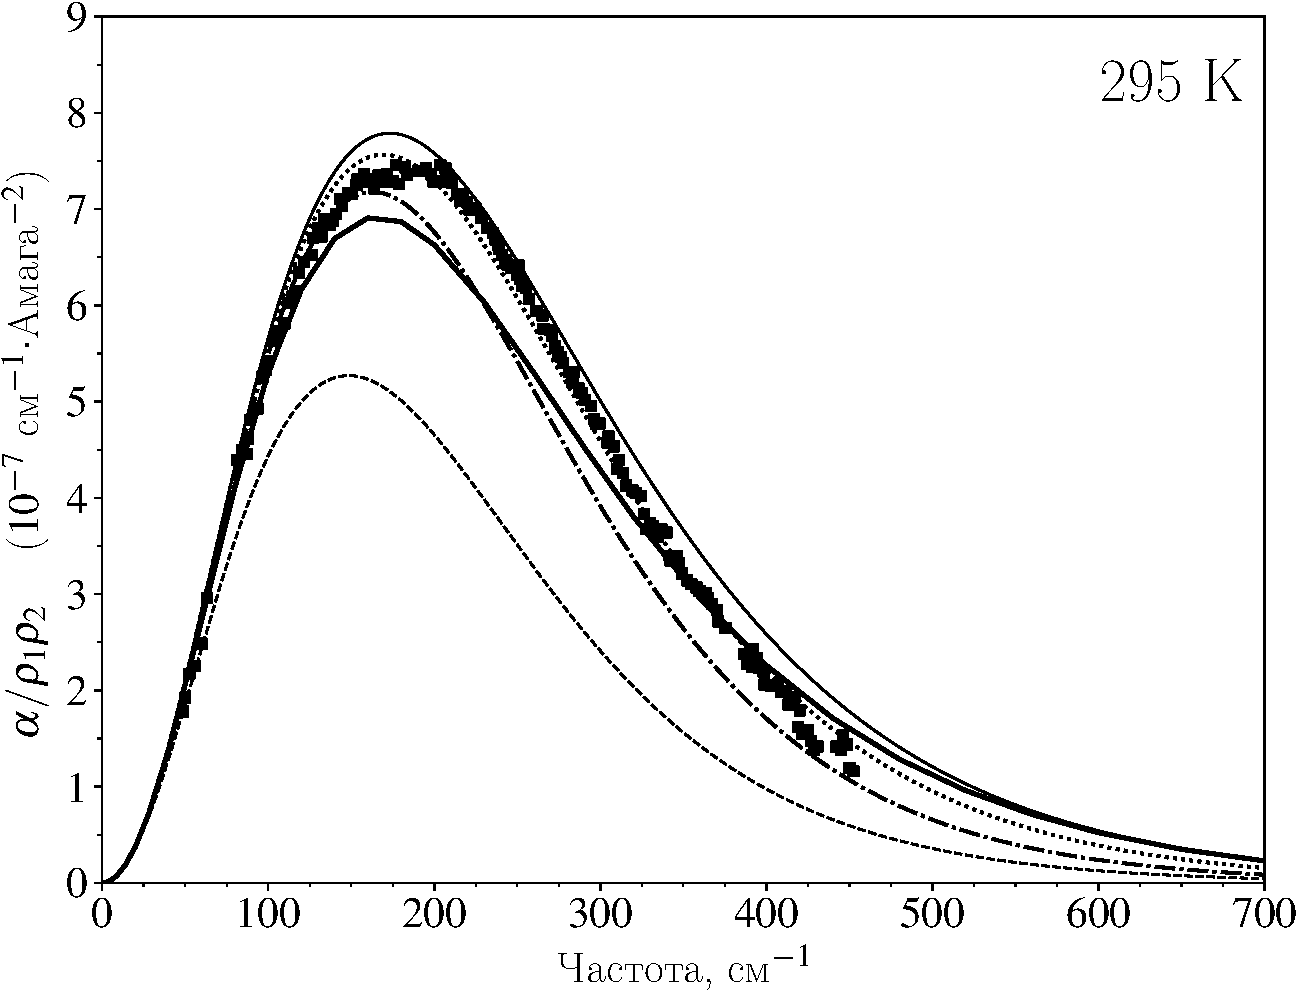
\includegraphics[width=0.7\linewidth]{./pictures/two_atom_spectra/desymmetrizations_295K-crop.pdf}
    \caption{Сравнение классического и квантового спектральных профилей для системы He$-$Ar с профилями, полученными в результате применения различных процедур десимметризации. Пунктиром обозначен классический профиль, сплошной толстой линией -- квантовый профиль \cite{buryak2014}, точками с пунктиром -- профиль, полученный в результате применения процедуры D1, точечной линией -- профиль, полученный в результате применения процедуры D2, сплошной линией -- профиль, полученный в результате применения процедуры D3. Квадратами обозначены экспериментальные данные \cite{bosomworth1965_part2}.}
    \label{fig:two-atom-desymmetrizations}
\end{figure}

Как известно, классические траектории обратимы во времени. Это свойство классических траекторий приводит к тому, что автокорреляционная функция дипольного момента $C(t)$ является симметричной функцией от времени \cite{frommhold}
\begin{gather}
    C(t) = C(-t).
\end{gather}

Классическая спектральная функция, получающаяся в результате применения преобразования Фурье к автокорреляционной функции, также оказывается симметричной функции частоты 
\begin{gather}
    J_\text{class.}(\omega) = J_\text{class.}(-\omega). \label{classical-detailed-balance}
\end{gather}

Однако квантовая спектральная функция удовлетворяет так называемому условию детального баланса \cite{frommhold} 
\begin{gather}
    J(-\omega) = J(\omega) \exp \lb -\frac{\hbar \omega}{\kb T} \rb, \label{detailed-balance}
\end{gather}
%
которое может быть получено из выражения \eqref{part1-spectral-function-definition} перестановкой индексов $j, k$. Условие детального баланса \eqref{detailed-balance} отражает разницу в заселенностях исходного и конечного состояний. Соотношение \eqref{classical-detailed-balance} называют классическим условием детального баланса. \par
Считается, что симметрийная разница между классической и квантовой спектральной функциями может быть устранена при помощи так называемой процедуры десимметризации. Предполагается, что классическую спектральную функцию можно определенным образом \enquote{десимметризовать} так, что функция, получившаяся в результате, будет удовлетворять квантовому условию детального баланса \cite{borysow1985phenomena}. Однако процедура десимметризации не может быть однозначна задана условием детального баланса: можно построить бесконечное количество процедур, которые будут приводить к спектральной функции, удовлетворяющей квантовому условию детального баланса \cite{frommhold}. Поэтому от процедуры десимметризации дополнительно требуют совпадения десимметризованного классического профиля с квантовым профилем -- в области дальних крыльев в особенности. \par
В литературе представлен набор различных процедур десимметризации \cite{borysow1985}. Некоторые из них устроены следующим образом:
\begin{gather}
    J_{D1}(\omega) = \frac{2}{1 + \exp \lb -\hbar \omega / \kb T \rb} J_\text{class}(\omega)  \\
    J_{D2}(\omega) = \frac{\hbar \omega}{\kb T} \frac{1}{1 - \exp \lb -\hbar \omega / \kb T \rb} J_\text{class}(\omega) \\
    J_{D3}(\omega) = \exp \lb \frac{\hbar \omega}{2 \kb T} \rb J_\text{class}(\omega)
\end{gather}
В литературе также используется преобразование Эгельстаффа \cite{egelstaff1962}; в настоящей работе мы его не использовали. 

\begin{figure}
    \centering
    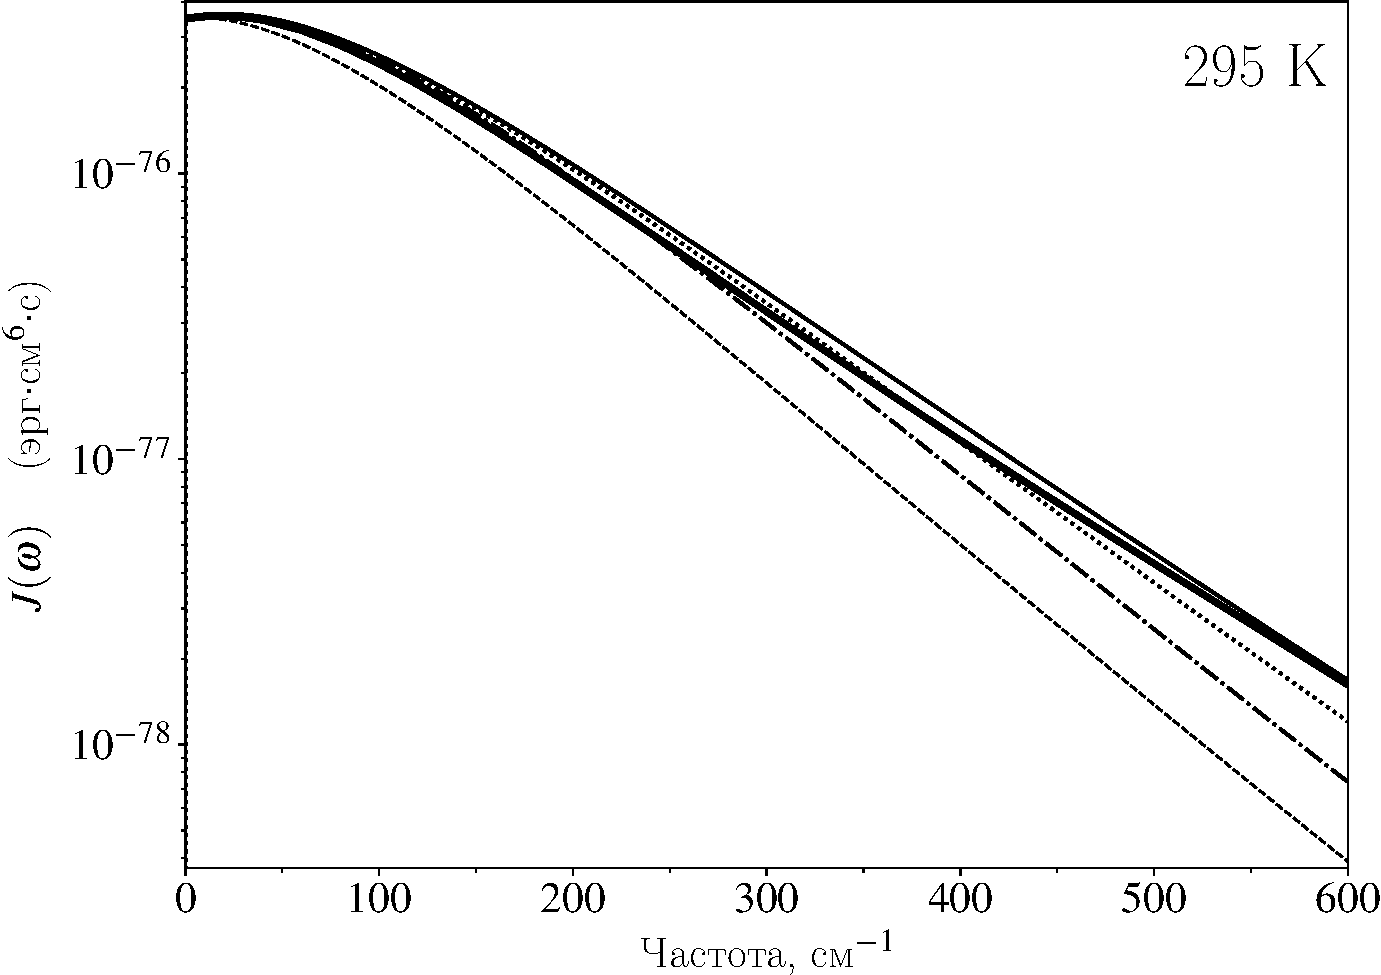
\includegraphics[width=0.7\linewidth]{./pictures/two_atom_spectra/spectral_function_desymmetrizations-crop.pdf}
    \caption{Сравнение крыльев классической, квантовой и десимметризованных спектральных функций системы He$-$Ar при температуре 295 K. Сплошной толстой линией обозначена квантовая спектральная функция \cite{buryak2014}; пунктиром -- классическая спектральная функция; пунктиром с точками -- спектральная функция, полученная в результате процедуры десимметризации D1; точечной линией -- спектральная функция, полученная в результате процедуры десимметризации D2; тонкой сплошной линией -- спектральная функция, полученная в результате процедуры десимметризации D3.}
    \label{fig:desymmetrisation-spectral-functions}
\end{figure}

Несложно убедиться, что приведенные процедуры десимметризации D1-D3 приводят к спектральным функциям, удовлетворяющим квантовому условию детального баланса. Продемонстрируем это на примере десимметризации D3, используя классическое правило детального баланса для $J_\text{class}(\omega)$:
\begin{gather}
    J_{D3}(\omega) = \exp \lb \frac{\hbar \omega}{2 \kb T} \rb J_\text{class}(\omega) \quad \implies \quad J_\text{class}(\omega) = \exp \lb -\frac{\hbar \omega}{2 \kb T} \rb J_{D3}(\omega), \label{d1} \\
    J_{D3}(-\omega) = \exp \lb -\frac{\hbar \omega}{2 \kb T} \rb J_\text{class}(-\omega) = \exp \lb -\frac{\hbar \omega}{2 \kb T} \rb J_\text{class}(\omega), \label{d2} \\
    J_{D3}(-\omega) = \exp \lb -\frac{\hbar \omega}{\kb T} \rb J_\text{D3}(\omega). \label{d3}
\end{gather}

Основываясь на рис. (\ref{fig:desymmetrisation-spectral-functions}), замечаем, что при малых частотах все спектральные функции ведут себя примерно одинаковым образом, однако с увеличением частоты различие между ними становится все больше. Одной из наиболее популярной в литературе является процедура D3. Спектральная функция, полученная в результате процедуры D3, переоценивает квантовую спектральную функцию в области крыла, однако считается, что около максимума спектра она дает наилучшую оценку. Сравнение при других температурах мы будем производить именно со спектром, полученным в результате процедуры D3. \par

\begin{figure}[H]
    \centering
    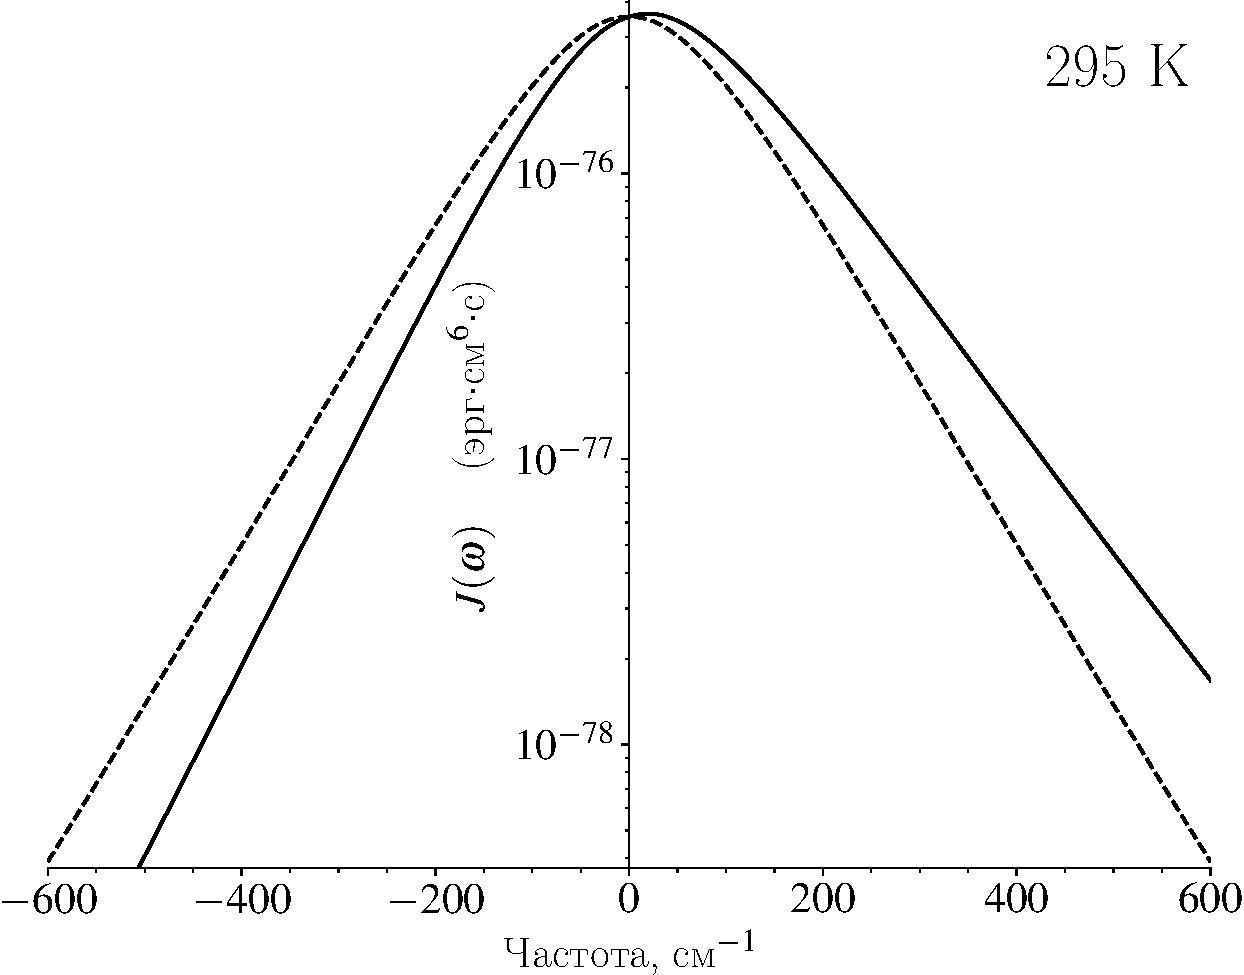
\includegraphics[width=0.49\linewidth]{./pictures/two_atom_spectra/spectral_function_d3-crop.pdf}
    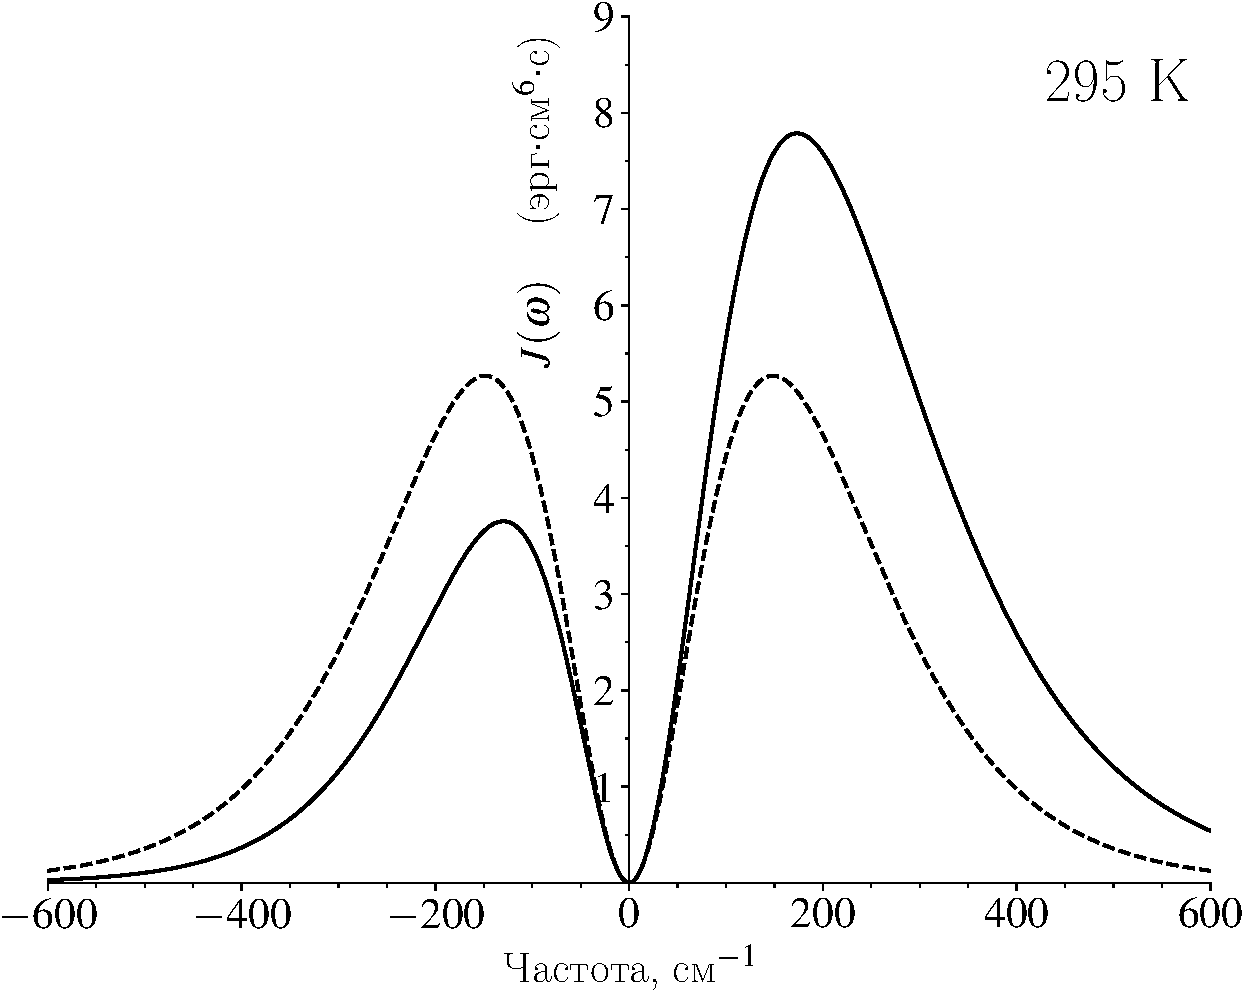
\includegraphics[width=0.49\linewidth]{./pictures/two_atom_spectra/spectrum_effect_d3-crop.pdf}
    \caption{Влияние десимметризации на спектральную функцию и спектральный профиль с учетом отрицательных частот. Пунктиром обозначены классические спектральная функция и профиль; сплошной линией -- полученные из классических в результате процедуры D3.}
    \label{fig:two-atom-d3-effect}
\end{figure}

Сравнение с экспериментальными данными на рис. (\ref{fig:two-atom-spectra}) показывает, что, несмотря на проблему выбора подходящей процедуры десимметризации, общее совпадение с экспериментальными данными оказывается неплохим. Отклонения между спектрами, полученными в результате применения различных процедур десимметризации, не превышает отклонения между квантовым профилем и экспериментальными данными. При всех температурах мы видим, что профиль, полученный в результате процедуры десимметризации D3, несколько превышает экспериментальные данные. \par 
Представленные на рис. (\ref{fig:two-atom-spectra}) спектральные профили получены в результате усреднения 2.000.000 траекторий. При всех температурах, кроме 240К, наблюдается достаточно близкое согласие с экспериментальными данными. При температуре 240К отклонение составляет порядка 10 \%, что попадает в стандартную погрешность экспериментальных данных, поэтому отклонение нельзя считать значимым. Также было обнаружено полное согласие с классическими спектрами, полученными в работе \cite{buryak2014} при помощи другой траекторной методики. 

\begin{figure}[H]
    \centering
    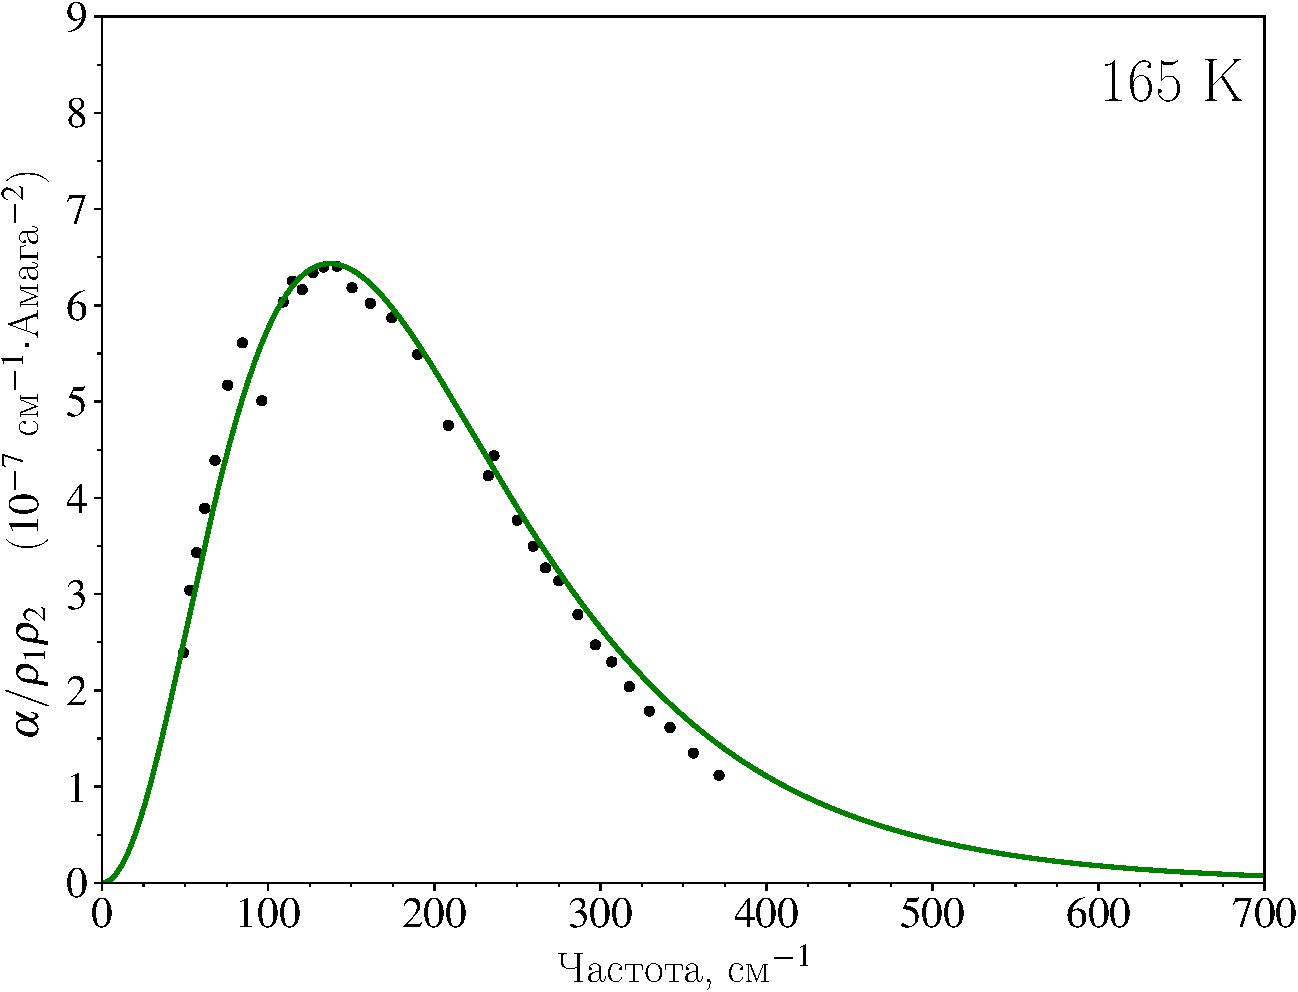
\includegraphics[width=0.49\linewidth]{./pictures/two_atom_spectra/alpha_165K-crop.pdf} 
    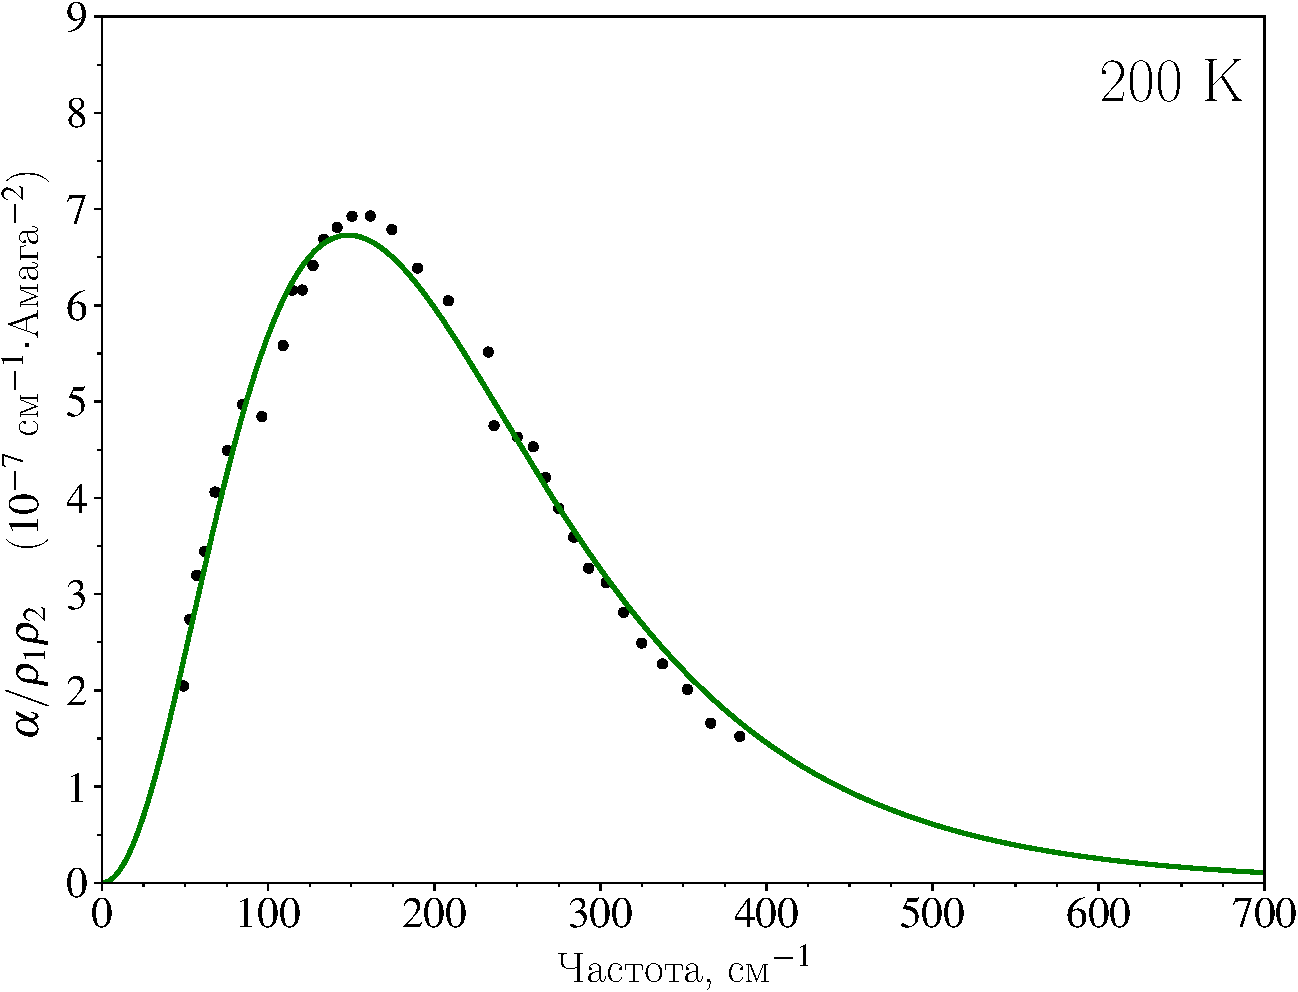
\includegraphics[width=0.49\linewidth]{./pictures/two_atom_spectra/alpha_200K-crop.pdf} \\
    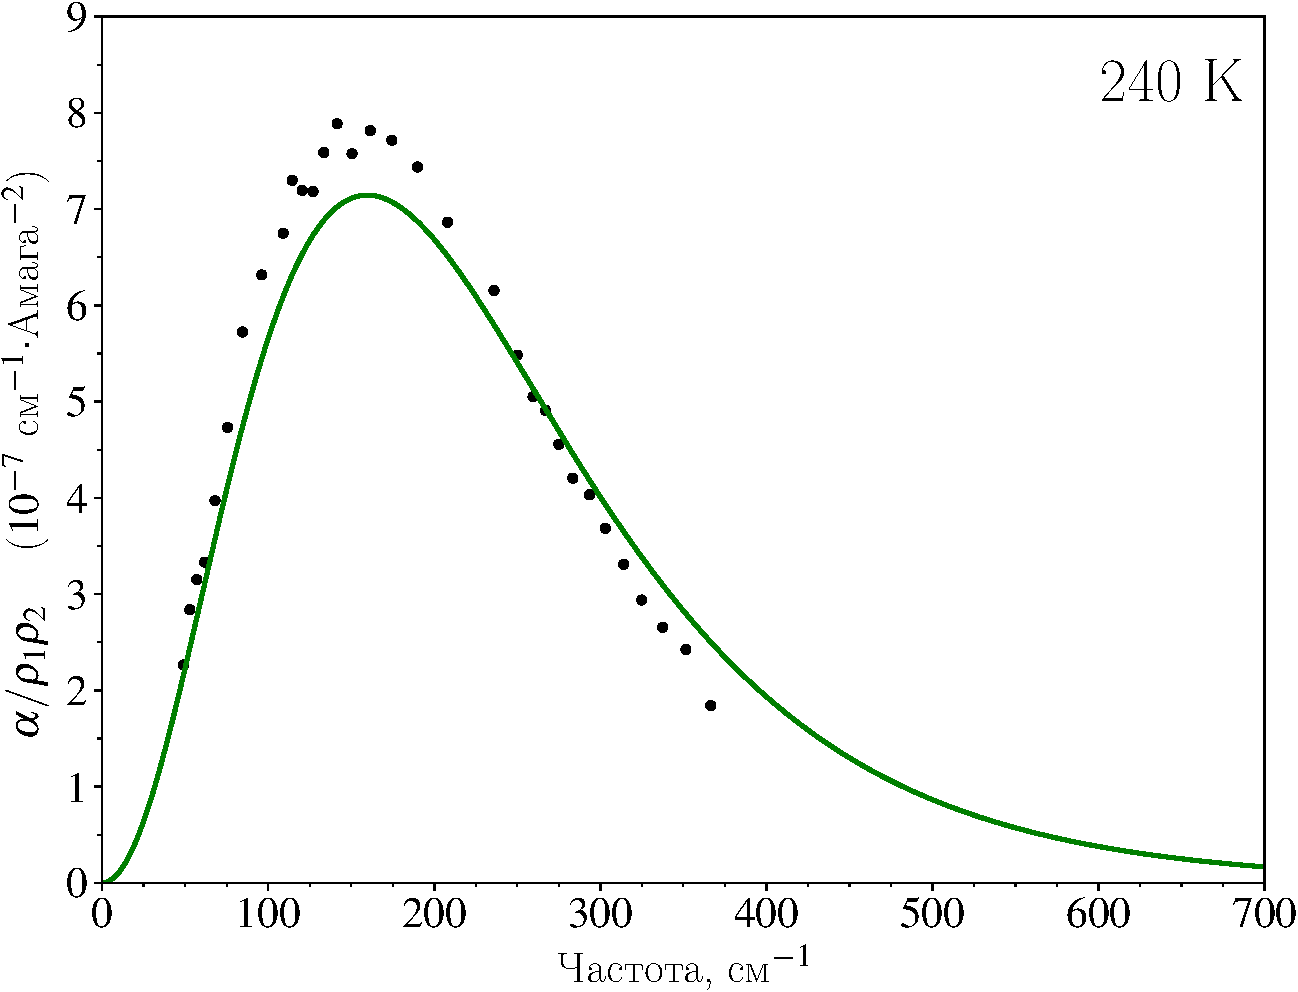
\includegraphics[width=0.49\linewidth]{./pictures/two_atom_spectra/alpha_240K-crop.pdf}
    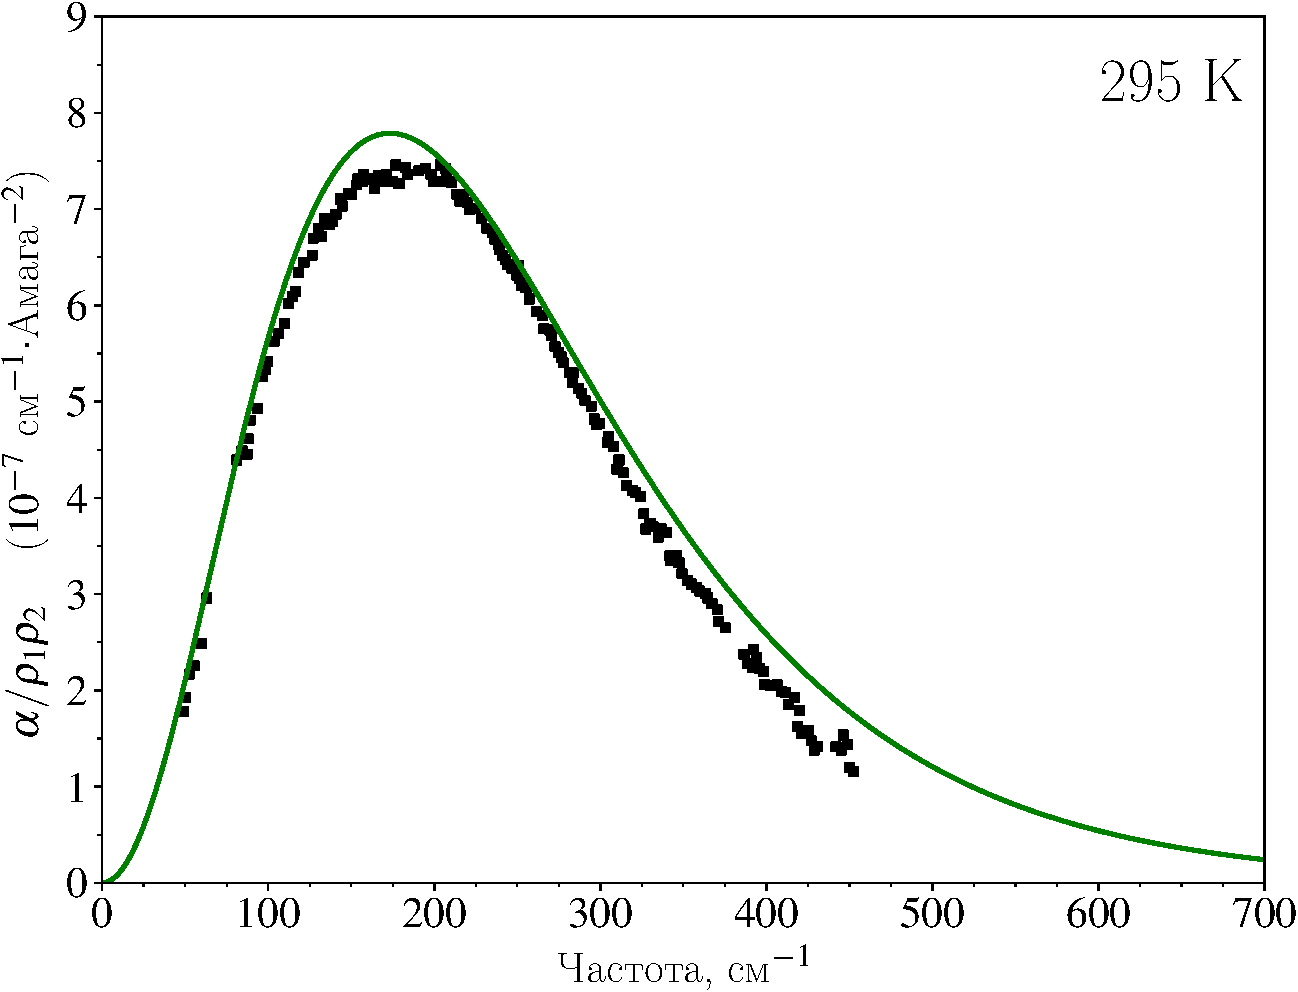
\includegraphics[width=0.49\linewidth]{./pictures/two_atom_spectra/alpha_295K-crop.pdf}
    \caption{Трансляционные спектры системы He$-$Ar при температурах 165K, 200K, 240K и 295K. Черными кружками обозначены экспериментальные данные из \cite{bukhtoyarova1977, bukhtoyarova1977_2, ryzhov1974}, квадратами -- из \cite{bosomworth1965_part2}.}
    \label{fig:two-atom-spectra}
\end{figure}

Сходимость расчета спектральной функции по Монте-Карло контролировалась при помощи спектральных моментов. Как отмечалось в теоретическом введении, спектральные моменты могут быть посчитаны как средние по фазовому пространству и как интегралы с использованием спектральной функции. Если на всех этапах траекторного расчета не допускаются систематические ошибки, то с увеличением количества траекторий моменты получаемой спектральной функции должны стремиться к моментам, полученным при усреднении по соотвествующей области фазового пространства. Так как начальные условия отбираются по области $H > 0$, то спектральные моменты для сравнения должны быть рассчитаны по соответствующей области фазового пространства. Расчет спектральных моментов производился по формулам \eqref{litreview-m0-phase-space}, \eqref{litreview-m2-phase-space}  при помощи адаптивного метода Монте-Карло \cite{hep}. В таблице (\ref{table:hear-moments}) представлены данные о сходимости спектральных профилей, представленных на рис. (\ref{fig:two-atom-spectra}). 

\begin{table}[H]
    \caption{Сравнение спектральных моментов, рассчитанных по фазовому пространству, с моментами по траекторным спектрам системы He$-$Ar}
    \begin{tabular}{c >{\centering}p{6cm} >{\centering}p{6cm} >{\centering}p{3cm}}
        \toprule
        $T$, K & Спектральные моменты $M_0$ (см$^{-1} \cdot$Амага$^{-2}$) и $M_2$ (см$^{-3} \cdot$Амага$^{-2}$) по фазовому пространству & Спектральные моменты $M_0$ (см$^{-1} \cdot$Амага$^{-2}$) и $M_2$ (см$^{-3} \cdot$Амага$^{-2}$) по траекторному спектру & Отклонение \tabularnewline
        \midrule
        \multirow{2}{*}{$165$}  & $3.113\cdot 10^{-6}$ & $3.110 \cdot 10^{-6}$ & $-0.1$ \%  \tabularnewline
                                & $3.061\cdot 10^{-2}$ & $3.077 \cdot 10^{-2}$ & $+0.5$ \%  \tabularnewline
        \midrule
        \multirow{2}{*}{$200$}  & $3.684\cdot 10^{-6}$ & $3.663 \cdot 10^{-6}$ & $-0.5$ \%  \tabularnewline
                                & $4.278\cdot 10^{-2}$ & $4.290 \cdot 10^{-2}$ & $+0.3$ \%  \tabularnewline
        \midrule
        \multirow{2}{*}{$240$}  & $4.347\cdot 10^{-6}$ & $4.337 \cdot 10^{-6}$ & $-0.2$ \%  \tabularnewline
                                & $5.912\cdot 10^{-2}$ & $5.983 \cdot 10^{-2}$ & $+1.2$ \%  \tabularnewline
        \midrule
        \multirow{2}{*}{$295$}  & $5.274\cdot 10^{-6}$ & $5.241 \cdot 10^{-6}$ & $-0.6$ \%  \tabularnewline
                                & $8.574\cdot 10^{-2}$ & $8.591 \cdot 10^{-2}$ & $+0.2$ \%  \tabularnewline
        \bottomrule
    \end{tabular}
    \label{table:hear-moments}
\end{table}



%\section{Квантовый подход к моделированию спектра}
%\section{Классический подход в лабораторной системе координат}
%\section{Вычислительные аспекты моделирования классических траекторий}

\chapter{Моделирование рототрансляционного столновительно-индуцированного спектра систем с вращательными степенями свободы}
\section{Существующие методы моделирования столкновительно-индуцированных спектров}
\section{Координаты Якоби}
\section{Гамильтониан в подвижной системе отсчета}
\section{Сравнение динамических систем уравнений}
\section{Классический подход в подвижной системе координат}
\section{Генерация начальных условий}
\section{Сравнение с экспериментальными данными}

\chapter{Выводы}

% можно попытаться докрутить свой bst-file, пока лень
%\bibliographystyle{mybst}
\bibliographystyle{unsrt}

\bibliography{biblio}

\end{document}
